%! Mode:: "TeX:UTF-8"
%! TEX program = xelatex
\documentclass[bwprint]{cumcmthesis}
\usepackage{ctex}
\usepackage{amsmath,amssymb,bm,booktabs,tabularx,array,longtable,enumitem}
\usepackage{graphicx}
\usepackage{float}
\usepackage{hyperref}
\usepackage[numbers,sort&compress]{natbib}
\usepackage{url}
\usepackage{subcaption}
\usepackage{tikz}
\usetikzlibrary{arrows.meta,positioning,shapes.geometric}
\setCJKfamilyfont{kai}[AutoFakeBold]{FandolKai-Regular.otf}

\floatstyle{ruled}
\newfloat{algorithm}{htbp}{loa}
\floatname{algorithm}{Algorithm}

\newcolumntype{C}{>{\centering\arraybackslash}X}
\newcolumntype{L}{>{\raggedright\arraybackslash}X}
\newcolumntype{R}{>{\raggedleft\arraybackslash}X}
\newcommand{\placeholderimage}[2]{%
\fbox{\parbox[c][#1][c]{0.86\textwidth}{\centering #2}}%
}
\lstdefinestyle{mcmpython}{
    language=Python,
    basicstyle=\zihao{6}\ttfamily,
    numbers=left,
    numberstyle=\tiny\color{gray},
    numbersep=0.8em,
    frame=single,
    breaklines=true,
    breakatwhitespace=false,
    showstringspaces=false,
    tabsize=4,
    captionpos=b
}

\title{板凳龙闹元宵\\基于等距螺线与分段几何约束的运动建模}
\tihao{A}
\baominghao{}
\schoolname{}
\membera{}
\memberb{}
\memberc{}
\supervisor{}
\yearinput{2024}
\monthinput{9}
\dayinput{5}
\makeatletter
\renewcommand*\mcm@commit@string@titlea{2024 高教社杯全国大学生数学建模竞赛}
\renewcommand*\mcm@numberpage@string@titlea{2024 高教社杯全国大学生数学建模竞赛}
\makeatother

\begin{document}
\maketitle
\pagenumbering{gobble}
\begin{abstract}
“板凳龙”由多节板凳通过把手首尾相连，运动过程中既受到螺线轨迹约束，又受到相邻把手距离、板凳实体宽度和调头空间边界的共同限制。本文围绕盘入、调头和盘出过程，建立以\textbf{等距螺线方程}、\textbf{极坐标弧长积分}、\textbf{逐节几何递推}、\textbf{有限宽度碰撞判定}和\textbf{速度比例缩放}为核心的统一模型，分别求解各时刻位置速度、无碰撞终止时刻、最小螺距、调头路径以及最大安全头速。

\textbf{针对问题一，}首先用\textbf{等距螺线方程}刻画半径随极角线性变化的盘入轨迹，再由极坐标参数曲线的弧长微元积分得到\textbf{螺线弧长函数}，据此反解龙头前把手的角参数；随后利用\textbf{相邻把手距离约束}逐节递推全队位置，并用\textbf{差分法}计算速度。模型生成了0--300 s内全部224个把手的位置和速度，位置表规模为 \textbf{449×302}，速度表规模为 \textbf{225×302}，相邻把手距离最大误差小于 \textbf{1.0e-11 m}。

\textbf{针对问题二，}将每节板凳视为有限宽度矩形，依据把手连线确定矩形轴线和法向，并采用\textbf{分离轴定理}判断非相邻板凳是否相交。再定义碰撞判定函数，通过\textbf{扫描}确定临界区间，并用\textbf{二分法}逼近首次碰撞时刻。无碰撞终止时刻为 \textbf{412.474 s}，首次碰撞板对为 \textbf{[0,8]}，终止状态下全队速度约在 \textbf{0.973--1.000 m/s} 之间。

\textbf{针对问题三，}在问题二碰撞判定思想的基础上，以龙头附近外侧角点到前方板凳轴线的最小距离作为接触判据。采用\textbf{变步长搜索}：以0.55 m为初始螺距逐步缩小，并在出现接触风险后减小步长继续逼近。满足盘入调头空间且不发生接触风险的最小螺距为 \textbf{0.45 m}。

\textbf{针对问题四，}在螺距1.7 m、调头空间半径4.5 m的条件下，以盘入螺线与调头圆的交点作为调头入点，并令盘出螺线与盘入螺线关于中心对称。根据\textbf{两圆弧相切模型}约束两段圆弧分别与盘入、盘出螺线相切、两圆弧相切以及半径比为2:1的几何关系，从而确定调头路径。两段圆弧半径分别为 \textbf{3.005 m} 和 \textbf{1.503 m}，调头路径长度为 \textbf{13.621 m}；同时输出调头前后100 s内每秒全队位置和速度。

\textbf{针对问题五，}在问题四固定路径上计算单位龙头速度下的全队速度矩阵。由于路径固定时各把手速度随龙头恒速成比例缩放，采用\textbf{单位头速归一化}得到最大速度放大倍数，并反推出龙头速度上界。单位头速下最大速度放大倍数为 \textbf{1.422}，限制把手为 \textbf{第1节龙身}，对应龙头最大恒定速度为 \textbf{1.406 m/s}。

\keywords{等距螺线\quad 几何递推\quad 碰撞判定\quad 二分搜索}
\end{abstract}


\pagenumbering{arabic}
\section{问题重述}
题目给出一条由223节板凳组成的“板凳龙”，要求在盘入、调头和盘出三个阶段中，结合把手约束、板凳宽度与调头空间边界，完成位置、速度、终止时刻、最小螺距、调头曲线和最大安全速度等计算。

从建模角度看，问题的核心不在于单个局部几何量，而在于如何把“龙头沿路径运动”与“整队板凳的相邻把手约束”统一到同一套参数化框架中。为此，本文先以等距螺线刻画盘入路径，再用逐节递推恢复全队状态；随后把每节板凳视作有限宽度矩形，利用碰撞检测判定运动可行性；最后围绕调头曲线长度与速度上限，分别转化为两圆弧几何构造和速度缩放问题。

\textbf{问题一：} 在螺距为0.55 m、龙头前把手速度恒为1 m/s的条件下，给出0--300 s内全部把手的位置和速度。

\textbf{问题二：} 沿问题一的盘入螺线继续运动，求首次发生碰撞前的终止时刻，并输出终止状态。

\textbf{问题三：} 在半径为4.5 m的调头空间内，求使龙头前把手能够盘入边界的最小螺距。

\textbf{问题四：} 在螺距为1.7 m的条件下，以螺线与调头圆的交点为调头入点，构造调头空间内的S形连接曲线。

\textbf{问题五：} 在问题四路径上，求满足所有把手速度均不超过2 m/s的龙头最大恒定速度。

\section{问题分析}
五个问题共享同一条主线：先确定龙头轨迹，再由把手间的几何约束回推整队状态，最后用碰撞与速度条件筛选可行解。

对问题一和问题二，关键在于建立“弧长--参数--坐标”的转换。龙头沿等距螺线运动时，弧长是时间的线性函数；只要能解出当前时刻对应的螺线参数，就能顺次恢复每节板凳的把手位置。问题二在此基础上增加了板凳实体宽度，因此不能只看把手中心线，而必须将每节板凳近似为有厚度的矩形，并检测非相邻板凳之间是否发生接触。

对问题三，最小螺距问题本质上是一个单变量可行性搜索。螺距越小，螺线越紧，整队越容易在调头空间边界附近产生干涉；因此可以把“给定螺距是否可行”作为判定函数，再用二分搜索逼近最小可行值。

对问题四，调头曲线由两段相切圆弧组成，且半径满足比例约束。入点由螺线与调头圆交点确定后，切线方向、圆弧半径和圆心角均可由几何关系推出。

对问题五，路径几何固定后，头部恒速会线性传递到全队各把手的速度幅值。于是只需先计算单位头速下的速度放大倍数，再通过“最大值不超过2 m/s”反推出头速上界即可。

\section{总体分析}
本题的关键在于把连续运动、几何约束和路径参数放进同一套语言中统一处理。Q1与Q2共用盘入螺线和把手递推，差别只是Q2进一步引入了板凳实体宽度；Q3则把螺距判定改写为角点到板凳轴线距离的临界搜索；Q4把调头部分抽象为固定交点下的两段相切圆弧；Q5在固定Q4路径后，通过速度缩放反推可接受的头速上限。

因此，全文的建模顺序应当是“先路径、后约束、再搜索”。先通过螺线弧长和递推关系确定运动状态，再通过几何判定筛选可行区域，最后对螺距或速度上界进行数值求解。这个顺序也与题目给出的五个问题自然对应。

\section{模型假设}
为使模型既可计算又不过度偏离题意，本文作如下假设。

\begin{enumerate}[itemindent=2em]
  \item 板凳在运动中视为刚体，单节板凳的几何尺寸在整个过程中保持不变。
  \item 每节板凳的两个把手中心位置固定，且相邻节之间仅通过把手连接。
  \item 盘入和盘出阶段的路径均可视为理想平面曲线，忽略弹性、摩擦和摆动等细节。
  \item 除题目允许的相邻连接外，任意两节非相邻板凳一旦实体相交即视为发生碰撞。
  \item 数值计算中的极小残差仅来自离散化与求根误差，不改变几何判定的结论。
\end{enumerate}

上述假设中，第4条是碰撞判定的核心，第5条用于说明数值结果的适用边界。它们共同保证后续结论具有明确的几何意义。

\section{符号说明}
\begin{table}[H]
\centering
\begin{tabularx}{\textwidth}{CL}
\toprule
符号 & 含义 \\
\midrule
$N$ & 板凳总节数，$N=223$ \\
$t$ & 时间，单位为s \\
$p$ & 螺距，单位为m \\
$v_H$ & 龙头前把手速度，单位为m/s \\
$P_i(t)$ & 第$i$个把手在时刻$t$的平面坐标 \\
$\ell_H$ & 龙头板前后把手中心距，$2.86$ m \\
$\ell_B$ & 普通板和龙尾板前后把手中心距，$1.65$ m \\
$r(\theta)$ & 等距螺线的极坐标半径函数 \\
$S(\theta)$ & 螺线从起点到参数$\theta$的弧长 \\
$R_T$ & 调头空间半径，$4.5$ m \\
$T_{\mathrm{stop}}$ & 问题二的无碰撞终止时刻 \\
$L_{\mathrm{turn}}$ & 调头曲线长度 \\
$v_{\max}$ & 问题五的龙头最大恒定速度 \\
\bottomrule
\end{tabularx}
\end{table}

其中，$P_i(t)$既可表示把手中心，也可在需要时表示与其绑定的板凳参考点，具体含义在各问题中保持一致。本文所有长度单位均为m，速度单位均为m/s，角度单位均为rad。

\section{问题一：盘入运动状态模型的建立与求解}
\subsection{问题一的建模思路}
问题一要求给出0--300 s内龙头、龙身和龙尾各把手的位置与速度。由于所有把手均约束在同一条盘入螺线上，而相邻板凳之间又由固定把手间距连接，因此可将问题拆为两个层次：先确定龙头前把手的螺线参数，再沿同一条曲线递推其余把手的参数。

本文采用极坐标描述螺线。原因在于，题目给出的轨迹本质上是等距螺线，其核心几何量是“半径随极角线性变化”；这一关系在极坐标下直接写成代数式，而在直角坐标中则会引入额外的旋转与曲率表达。故位置求解的关键量由二维坐标降为单一参数$\theta$。

\subsection{等距螺线方程的建立}
设螺线中心为原点$O$，$x$轴水平向右，$y$轴竖直向上。根据题图约定，点A位于正$x$轴上，龙头沿顺时针方向向内盘入。等距螺线满足
\[
r(\theta+2\pi)-r(\theta)=p.
\]
若取半径关于极角线性变化，则有
\[
r(\theta)=b\theta,\qquad b=\frac{p}{2\pi}.
\]
问题一中$p=0.55$ m，所以
\[
b=\frac{0.55}{2\pi}.
\]
将极坐标转为直角坐标，得到把手中心的位置表达式
\[
\begin{cases}
x(\theta)=r(\theta)\cos\theta,\\
y(\theta)=r(\theta)\sin\theta.
\end{cases}
\]
因此，一旦确定某一把手对应的螺线参数$\theta$，其平面位置就被唯一确定。

为直观说明上述极坐标建模过程，等距螺线的几何要素示意图如下。

\begin{figure}[H]
\centering
\placeholderimage{5.4cm}{
图位预留：等距螺线极坐标建模示意图。\\[0.4em]
图中标出极点$O$、极角$\theta$、半径$r$、螺距$p$，\\
并标明$r=b\theta$与相邻两圈半径差$p$之间的关系。
}
\caption{等距螺线极坐标建模示意}
\label{fig:q1-spiral-model}
\end{figure}

\subsection{龙头前把手的弧长关系}
题目给定龙头前把手的速度为1 m/s。对于参数曲线
\[
x(\theta)=b\theta\cos\theta,\qquad y(\theta)=b\theta\sin\theta,
\]
其导数为
\[
\frac{dx}{d\theta}=b\cos\theta-b\theta\sin\theta,\qquad
\frac{dy}{d\theta}=b\sin\theta+b\theta\cos\theta.
\]
故弧长微元满足
\[
ds=\sqrt{\left(\frac{dx}{d\theta}\right)^2+\left(\frac{dy}{d\theta}\right)^2}\,d\theta
=b\sqrt{1+\theta^2}\,d\theta.
\]
于是从0到$\theta$的弧长函数为
\[
S(\theta)=\int_0^\theta b\sqrt{1+u^2}\,du
=\frac{b}{2}\Bigl[\theta\sqrt{\theta^2+1}+\operatorname{asinh}(\theta)\Bigr].
\]
该函数把螺线参数与沿曲线行进距离联系起来，因此龙头位置可由弧长反解得到。

\subsection{初始角$\theta_0$的确定}
题目说明龙头从第16圈处开始盘入。等距螺线绕原点一圈对应极角变化$2\pi$，第16圈对应
\[
\theta_0=16\times2\pi=32\pi.
\]
在本文的坐标约定下，$\theta_0=32\pi$对应正$x$轴方向，与题图中A点位于正$x$轴一致。由于龙头顺时针向内运动，半径随时间减小，等价于$\theta$随时间减小。

设龙头前把手在时刻$t$的参数为$\theta_H(t)$，则
\[
S(\theta_0)-S\!\left(\theta_H(t)\right)=v_H t,\qquad v_H=1.
\]
即
\[
S\!\left(\theta_H(t)\right)=S(\theta_0)-v_H t.
\]
由此得到一元单调方程。求得$\theta_H(t)$后，再代入坐标转换式即可恢复龙头前把手的位置。

\subsection{相邻把手递推模型}
龙头前把手确定后，其余把手必须满足相邻把手中心距离固定。龙头板的前后把手中心距为
\[
\ell_H=3.41-2\times0.275=2.86\ \text{m},
\]
普通龙身板和龙尾板的前后把手中心距为
\[
\ell_B=2.20-2\times0.275=1.65\ \text{m}.
\]

相邻把手、板凳实体与中心线之间的几何关系示意图如下，该图用于说明后续递推约束与碰撞矩形模型的共同几何来源。

\begin{figure}[H]
\centering
\placeholderimage{5.0cm}{
图位预留：相邻把手与板凳实体几何关系图。\\[0.4em]
图中标出前后把手中心、把手间距$\ell_H,\ell_B$、板长、板宽$w$、\\
把手孔到板端的外延，以及由把手连线确定的板凳中心轴。
}
\caption{相邻把手与板凳实体的几何关系示意}
\label{fig:q1-bench-geometry}
\end{figure}

记第$i$个把手在时刻$t$对应的螺线参数为$\theta_i(t)$，位置为
\[
P_i(t)=\bigl(x(\theta_i(t)),y(\theta_i(t))\bigr).
\]
已知$P_i(t)$后，第$i+1$个把手仍位于同一条螺线上，且满足
\[
\left\|P_{i+1}(t)-P_i(t)\right\|_2=d_i,
\qquad
d_i=
\begin{cases}
\ell_H, & i=0,\\
\ell_B, & i=1,2,\ldots,222.
\end{cases}
\]
展开得
\[
\left[x(\theta_{i+1})-x(\theta_i)\right]^2+
\left[y(\theta_{i+1})-y(\theta_i)\right]^2=d_i^2.
\]
由于板凳龙由头至尾单向排布，后一把手在螺线上对应更外侧的参数值，即$\theta_{i+1}>\theta_i$。在该单调区间内求解上式，可排除非物理解。于是，问题一的几何状态由“路径约束+间距约束”唯一确定。

\subsection{速度计算}
对后续把手，速度按相邻时刻的轨迹长度差分得到。若记第$i$个把手在相邻时刻的位置为$P_i(t-\Delta t)$和$P_i(t+\Delta t)$，则可用中心差分近似
\[
v_i(t)\approx
\frac{\left\|P_i(t+\Delta t)-P_i(t-\Delta t)\right\|_2}{2\Delta t}.
\]
端点时刻使用单侧差分。该做法与逐秒输出要求一致，也避免了显式求解隐函数导数。

\subsection{求解流程}
\begin{algorithm}[H]
\caption{问题一逐时刻位置与速度求解流程}
\label{alg:q1-state}
\textbf{Input:} 螺距$p=0.55$，整数时刻$t=0,1,\ldots,300$，把手间距$d_i$。\\
\textbf{Output:} 全部把手的位置表与速度表。
\begin{enumerate}[label=\arabic*:, leftmargin=2.6em, itemsep=0.2em]
\item 令$b=p/(2\pi)$，建立等距螺线$r(\theta)=b\theta$。
\item 对每个时刻$t$，求解弧长方程$S(\theta_0)-S(\theta_H(t))=v_Ht$，得到龙头前把手参数$\theta_H(t)$。
\item 对$i=1,\ldots,223$，在$\theta_i>\theta_{i-1}$分支上求解$\|P_i(t)-P_{i-1}(t)\|_2=d_i$。
\item 将所有$\theta_i(t)$代入坐标变换，得到$(x_i(t),y_i(t))$。
\item 对离散位置序列作差分，得到各把手速度$v_i(t)$。
\item \textbf{return} 位置表与速度表。
\end{enumerate}
\end{algorithm}
上述流程把“轨迹反解”和“链式递推”分离开来，便于逐时刻稳定求解。

根据该流程得到的板凳龙在盘入螺线上的某一时刻整体排布示意图如下。

\begin{figure}[H]
\centering
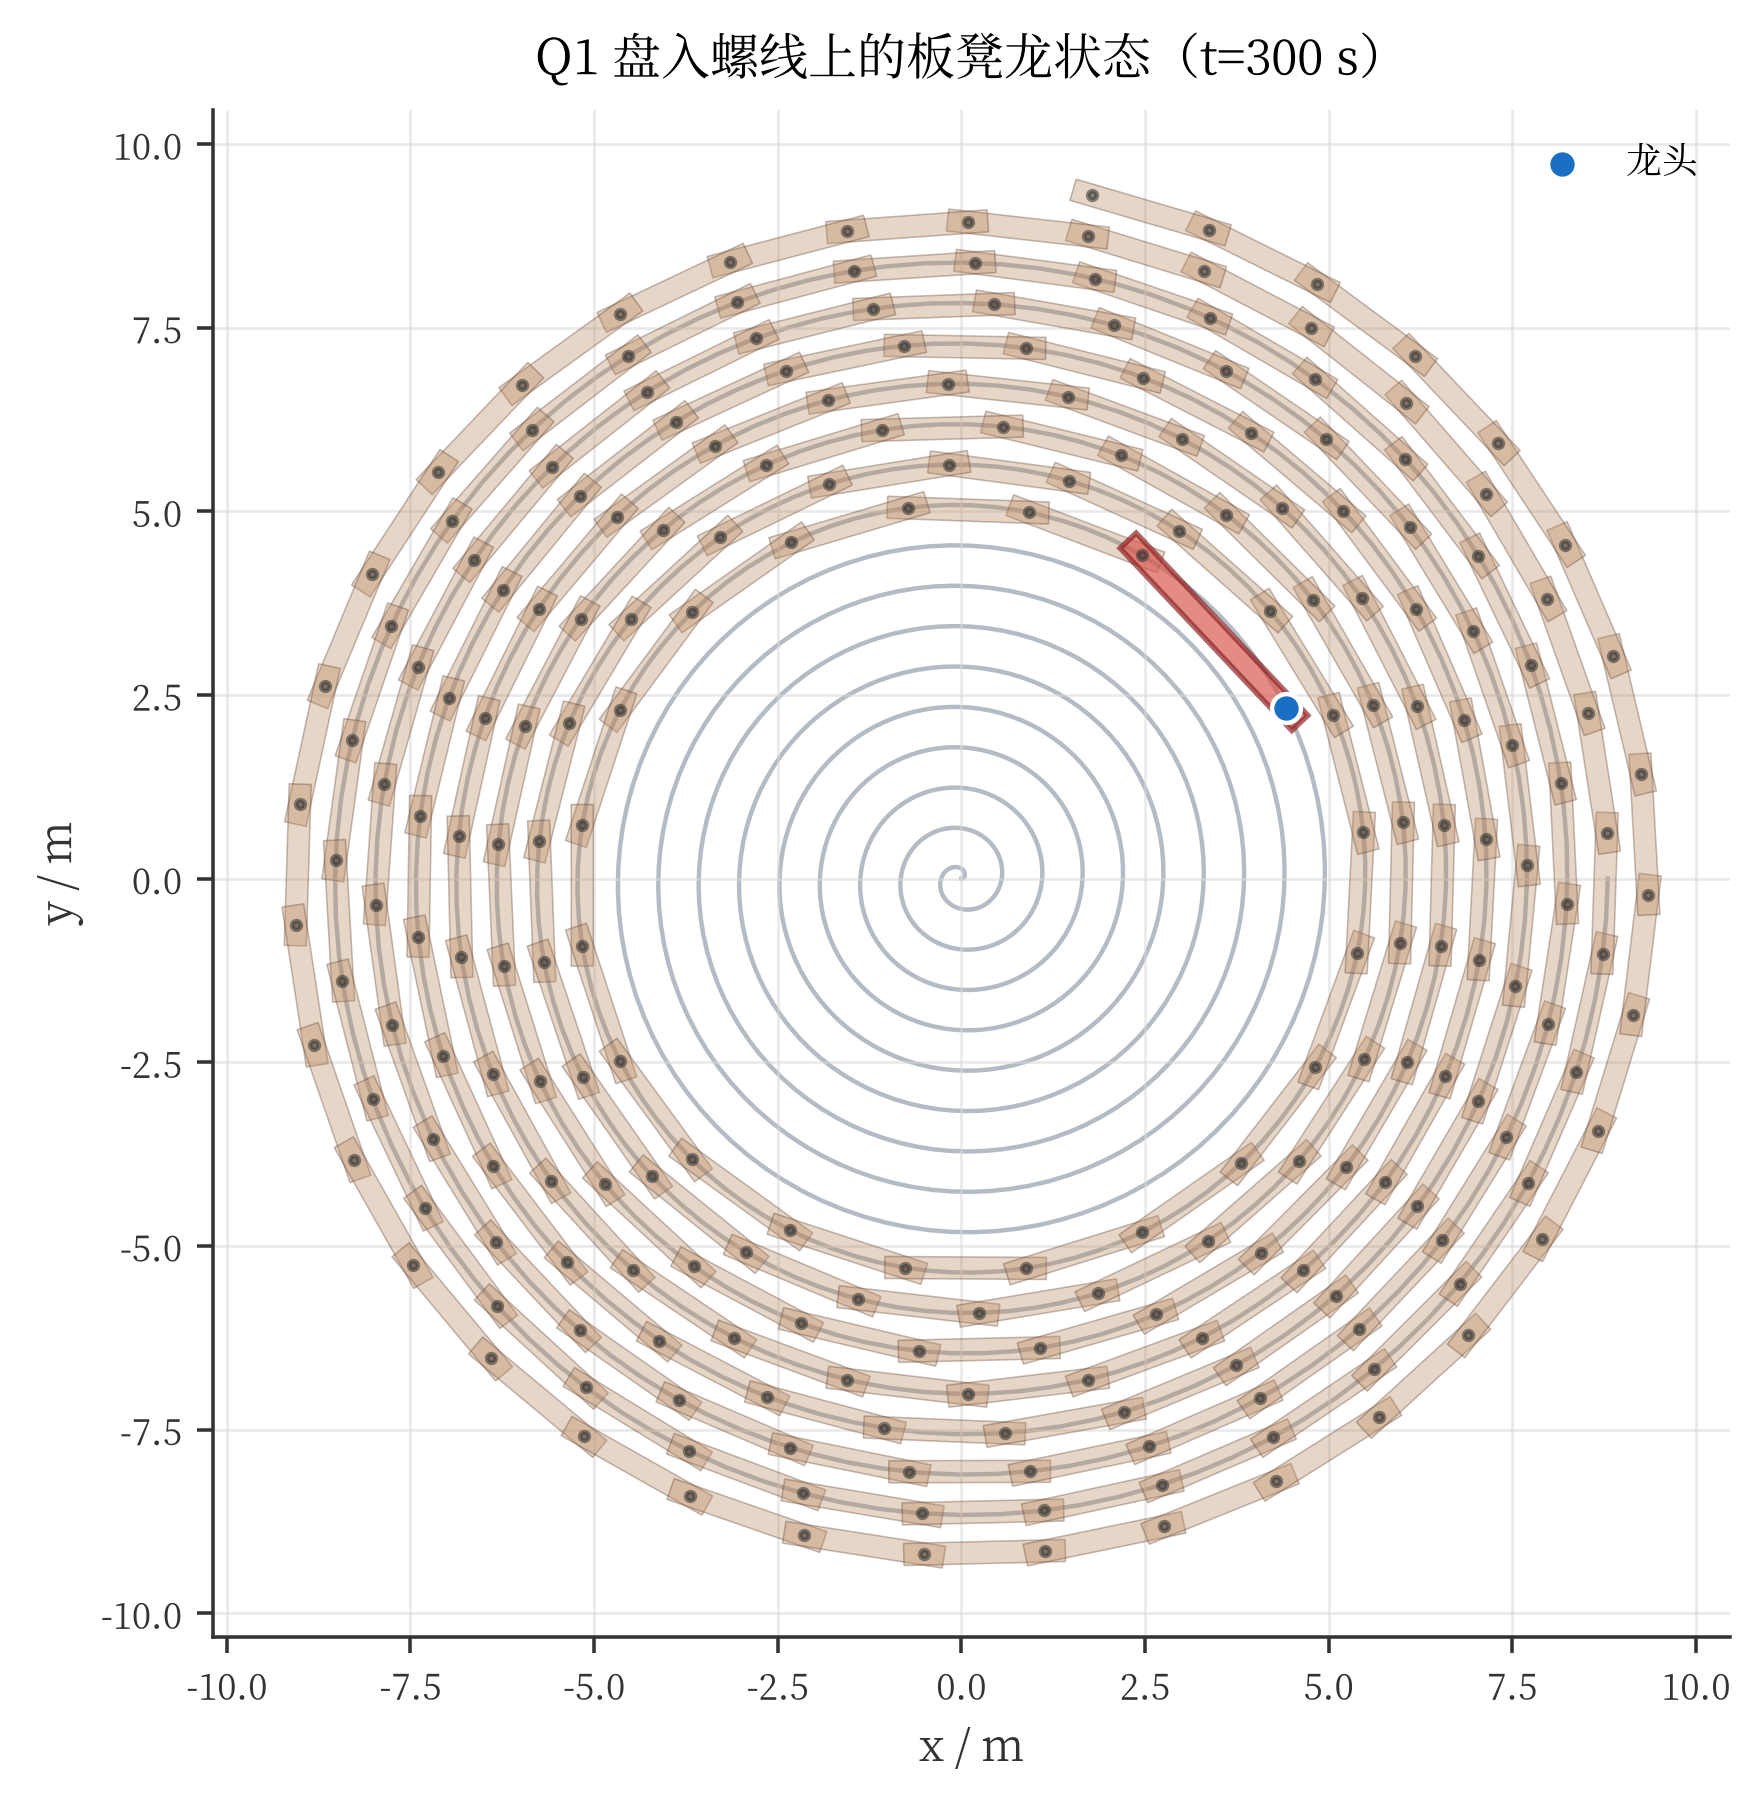
\includegraphics[width=0.92\textwidth]{figures/python/q1_spiral_bench_snapshot.png}
\caption{板凳龙在盘入螺线上的运动状态截取}
\label{fig:q1-spiral-snapshot}
\end{figure}

\subsection{结果分析}
按上述模型输出的0--300 s数据中，位置表规模为449行、302列，速度表规模为225行、302列，覆盖全部224个把手和301个整数时刻。相邻把手距离的最大误差为
\[
8.32\times10^{-12}\ \text{m},
\]
平均绝对误差为
\[
4.64\times10^{-14}\ \text{m}.
\]
这说明逐节递推在数值上很好地保持了板凳连接约束。与稠密折线基线在0 s、60 s、120 s、180 s、240 s和300 s处比较，最大坐标差为$0.0153$ m，说明模型输出与离散路径近似结果保持一致。

\begin{table}[H]
\centering
\caption{问题一位置抽样表}
\label{tab:q1-position}
\begingroup
\small
\setlength{\tabcolsep}{2pt}
\begin{tabularx}{\textwidth}{lCCCCCC}
\toprule
项目 & 0 s & 60 s & 120 s & 180 s & 240 s & 300 s\\
\midrule
龙头 $x$ (m) & 8.800000 & 5.799209 & -4.084887 & -2.963609 & 2.594494 & 4.420274\\
龙头 $y$ (m) & 0.000000 & -5.771092 & -6.304479 & 6.094780 & -5.356743 & 2.320429\\
第1节龙身 $x$ (m) & 8.363824 & 7.456758 & -1.445473 & -5.237118 & 4.821221 & 2.459489\\
第1节龙身 $y$ (m) & 2.826544 & -3.440399 & -7.405883 & 4.359627 & -3.561949 & 4.402476\\
第51节龙身 $x$ (m) & -9.518732 & -8.686317 & -5.543150 & 2.890455 & 5.980011 & -6.301346\\
第51节龙身 $y$ (m) & 1.341137 & 2.540108 & 6.377946 & 7.249289 & -3.827758 & 0.465829\\
第101节龙身 $x$ (m) & 2.913983 & 5.687116 & 5.361939 & 1.898794 & -4.917371 & -6.237722\\
第101节龙身 $y$ (m) & -9.918311 & -8.001384 & -7.557638 & -8.471614 & -6.379874 & 3.936008\\
第151节龙身 $x$ (m) & 10.861726 & 6.682311 & 2.388757 & 1.005154 & 2.965378 & 7.040740\\
第151节龙身 $y$ (m) & 1.828753 & 8.134544 & 9.727411 & 9.424751 & 8.399721 & 4.393013\\
第201节龙身 $x$ (m) & 4.555102 & -6.619664 & -10.627211 & -9.287720 & -7.457151 & -7.458662\\
第201节龙身 $y$ (m) & 10.725118 & 9.025570 & 1.359847 & -4.246673 & -6.180726 & -5.263384\\
龙尾（后） $x$ (m) & -5.305444 & 7.364557 & 10.974348 & 7.383896 & 3.241051 & 1.785033\\
龙尾（后） $y$ (m) & -10.676584 & -8.797992 & 0.843473 & 7.492370 & 9.469336 & 9.301164\\
\bottomrule
\end{tabularx}
\endgroup
\end{table}

\begin{table}[H]
\centering
\caption{问题一速度抽样表}
\label{tab:q1-speed}
\begingroup
\small
\setlength{\tabcolsep}{2pt}
\begin{tabularx}{\textwidth}{lCCCCCC}
\toprule
项目 & 0 s & 60 s & 120 s & 180 s & 240 s & 300 s\\
\midrule
龙头 (m/s) & 1.000000 & 1.000000 & 1.000000 & 1.000000 & 1.000000 & 1.000000\\
第1节龙身 (m/s) & 0.999971 & 0.999961 & 0.999945 & 0.999917 & 0.999859 & 0.999709\\
第51节龙身 (m/s) & 0.999742 & 0.999662 & 0.999538 & 0.999331 & 0.998941 & 0.998065\\
第101节龙身 (m/s) & 0.999575 & 0.999453 & 0.999269 & 0.998971 & 0.998435 & 0.997302\\
第151节龙身 (m/s) & 0.999448 & 0.999299 & 0.999078 & 0.998727 & 0.998115 & 0.996861\\
第201节龙身 (m/s) & 0.999348 & 0.999180 & 0.998935 & 0.998551 & 0.997894 & 0.996574\\
龙尾（后） (m/s) & 0.999311 & 0.999136 & 0.998883 & 0.998489 & 0.997816 & 0.996478\\
\bottomrule
\end{tabularx}
\endgroup
\end{table}

由表\ref{tab:q1-speed}可见，龙头速度保持为1 m/s，其余关键把手速度随时间略有下降。为更直观比较不同位置把手的速度变化，关键把手速度随时间变化曲线如下。

\begin{figure}[H]
\centering
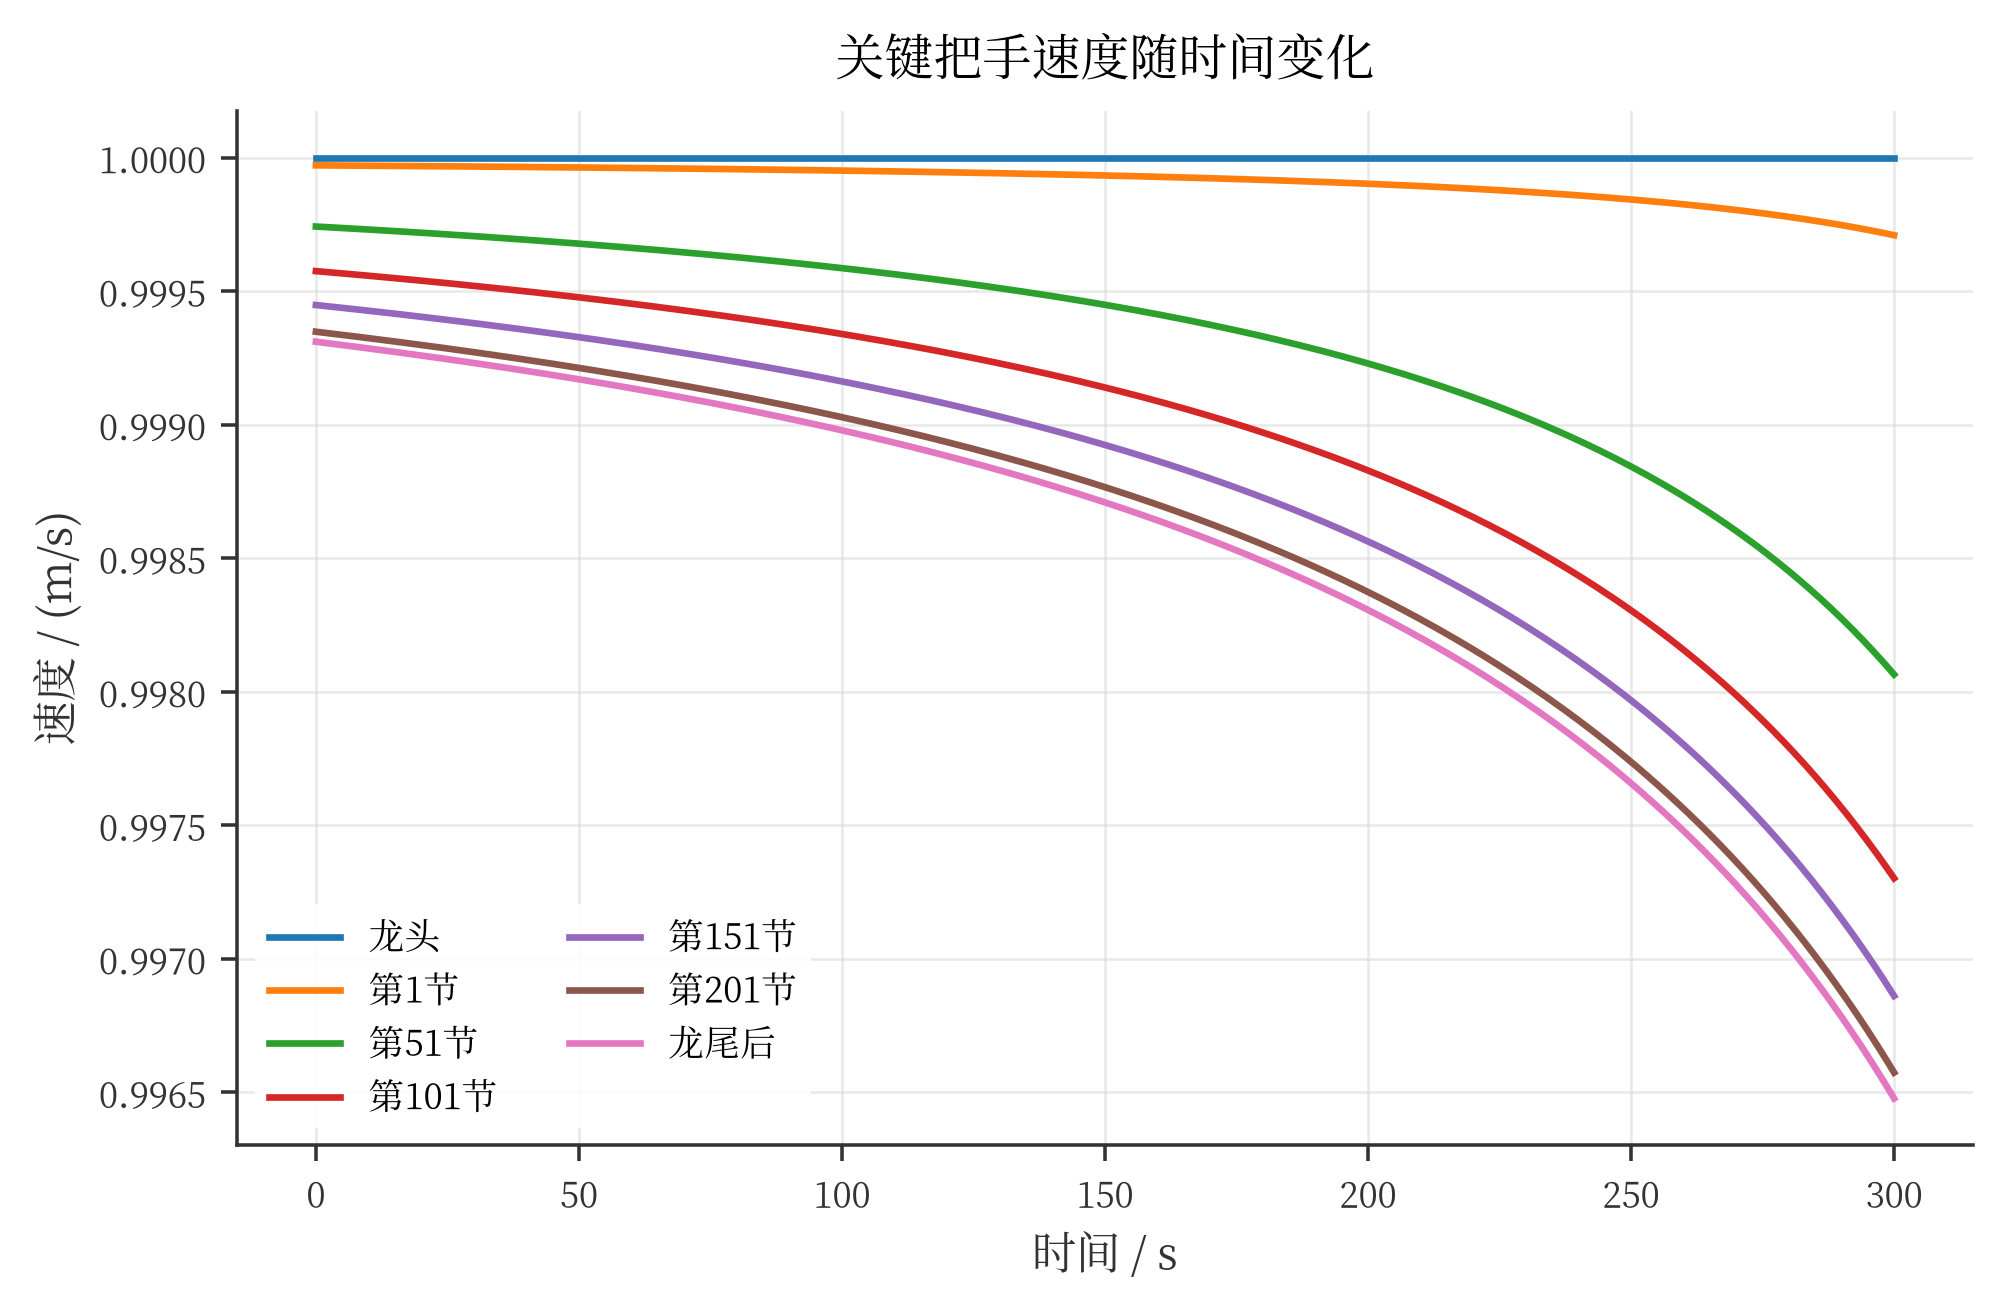
\includegraphics[width=0.88\textwidth]{figures/python/q1_key_handle_speed_time.png}
\caption{关键把手速度随时间变化}
\label{fig:q1-key-speed-time}
\end{figure}

因此，问题一的等距螺线弧长模型既满足题目对位置和速度输出的要求，也为后续碰撞判定、最小螺距搜索和调头路径建模提供了统一的几何基础。

\section{问题二：无碰撞终止时刻的判定}
\subsection{问题二的建模动机}
问题二要求在问题一的盘入轨迹上确定无碰撞终止时刻。若仍只看把手中心线，就只能得到点与点的相对位置，而无法判断实体板凳是否接触；因此必须把每节板凳视为具有长度和宽度的平面刚体。由此，问题二实质上转化为一个几何可行域的临界判定问题。

题目给出的板长、板宽和把手孔中心距板端的偏移量，足以把每节板凳近似成一个有限宽度矩形。该矩形的轴线由前后把手中心连线确定，宽度取0.30 m。于是“是否碰撞”就可以被写成两个矩形是否有交集的问题。

\subsection{矩形板凳模型}
对第$i$节板凳，设前后把手中心分别为$P_i^{\mathrm{f}}$和$P_i^{\mathrm{b}}$，则板凳中心轴方向向量可写为
\[
\bm{u}_i=\frac{P_i^{\mathrm{f}}-P_i^{\mathrm{b}}}{\|P_i^{\mathrm{f}}-P_i^{\mathrm{b}}\|_2},
\]
对应的法向单位向量记为$\bm{v}_i$。于是，第$i$节板凳可表示为
\[
\mathcal{R}_i=\left\{P_i^{\mathrm{c}}+\xi \bm{u}_i+\eta \bm{v}_i:
\ |\xi|\le \frac{L_i}{2},\ |\eta|\le \frac{w}{2}\right\},
\]
其中$P_i^{\mathrm{c}}$为板凳中心点，$L_i$为该节板凳沿轴线方向的有效长度，$w=0.30$ m 为板宽。把手中心到板端的偏移固定为0.275 m，因此有效长度可由把手间距与两端外延共同确定。

\subsection{碰撞约束的数学表达}
问题二只检查非相邻板凳。若两节板凳相邻，则它们本就通过把手连接，不应视作碰撞；若两节板凳不相邻，则要求其矩形区域互不相交。故判定条件可写为
\[
\mathcal{R}_i\cap \mathcal{R}_j=\varnothing,\qquad |i-j|>1.
\]

分离轴定理指出：两个凸多边形不相交，当且仅当存在一条直线，使得两个多边形在该直线法向上的投影区间互不重叠。由于矩形是凸多边形，且其可能的分离轴只需取自两矩形的边法向方向，因此本题中每一对矩形板凳只需检查四个单位方向
\[
\mathcal{E}_{ij}=\{\bm{u}_i,\bm{v}_i,\bm{u}_j,\bm{v}_j\}.
\]
对任意单位方向$\bm{e}\in\mathcal{E}_{ij}$，第$i$节板凳在该方向上的投影区间可写为
\[
I_i(\bm{e})=
\left[
P_i^{\mathrm{c}}\cdot\bm{e}-\rho_i(\bm{e}),
P_i^{\mathrm{c}}\cdot\bm{e}+\rho_i(\bm{e})
\right],
\]
其中投影半径为
\[
\rho_i(\bm{e})
=\frac{L_i}{2}\left|\bm{u}_i\cdot\bm{e}\right|
+\frac{w}{2}\left|\bm{v}_i\cdot\bm{e}\right|.
\]
于是，两节非相邻板凳不碰撞等价于至少存在一个候选方向使投影区间分离，即
\[
\exists\,\bm{e}\in\mathcal{E}_{ij},\quad
\left|
\left(P_i^{\mathrm{c}}-P_j^{\mathrm{c}}\right)\cdot\bm{e}
\right|
>
\rho_i(\bm{e})+\rho_j(\bm{e}).
\]
反之，若对四个候选方向均有
\[
\left|
\left(P_i^{\mathrm{c}}-P_j^{\mathrm{c}}\right)\cdot\bm{e}
\right|
\le
\rho_i(\bm{e})+\rho_j(\bm{e}),
\qquad \forall\,\bm{e}\in\mathcal{E}_{ij},
\]
则两矩形在所有候选轴上的投影均重叠，判定为发生实体碰撞。由此，时刻$t$下的全队无碰撞约束可写为
\[
\forall\, i,j,\ |i-j|>1,\quad
\exists\,\bm{e}\in\mathcal{E}_{ij}(t)\ \text{使上式严格分离成立}.
\]
这就是分离轴定理在本题中的具体应用：先由把手位置确定每节板凳的矩形区域，再对所有非相邻矩形板凳逐对检查四个投影方向。

为了直观呈现“投影区间分离即不碰撞”的判定方式，分离轴定理在矩形板凳上的应用示意图如下。

\begin{figure}[H]
\centering
\placeholderimage{5.4cm}{
图位预留：分离轴定理矩形投影示意图。\\[0.4em]
图中标出两块非相邻板凳矩形、候选方向$\bm u_i,\bm v_i,\bm u_j,\bm v_j$，\\
以及两矩形在某一候选轴上的投影区间$I_i(\bm e),I_j(\bm e)$。
}
\caption{分离轴定理在矩形板凳碰撞判定中的应用示意}
\label{fig:q2-sat}
\end{figure}

\subsection{临界时刻与单调性}
设
\[
\chi(t)=
\begin{cases}
0, & \text{时刻 } t \text{ 无碰撞},\\
1, & \text{时刻 } t \text{ 发生碰撞}.
\end{cases}
\]
则终止时刻可定义为
\[
T_{\mathrm{stop}}=\sup\{t:\chi(t)=0\}.
\]
在题设盘入过程中，龙头持续向内，板凳间距只会逐渐压缩，因此$\chi(t)$在临界附近呈现从0到1的单调跃迁。这一结构意味着：只要找到一个无碰撞时刻和一个碰撞时刻，就能在两者之间逼近临界点。

因此，我们采用扫描加二分的方式确定首次碰撞时刻。首先按时间顺序扫描若干采样点，找到最后一个满足$\chi(t)=0$的时刻$t^{-}$和第一个满足$\chi(t)=1$的时刻$t^{+}$，从而得到包含临界时刻的区间$[t^{-},t^{+}]$。随后取中点$t_m=(t^{-}+t^{+})/2$并重新计算$\chi(t_m)$：若$\chi(t_m)=0$，则令$t^{-}=t_m$；若$\chi(t_m)=1$，则令$t^{+}=t_m$。重复该过程，直到区间长度小于给定容差，此时$t^{-}$即作为无碰撞终止时刻的数值近似。

\subsection{求解流程}
\begin{algorithm}[H]
\caption{问题二首次碰撞时刻搜索流程}
\label{alg:q2-collision}
\textbf{Input:} 问题一得到的把手轨迹，板凳宽度和把手间距。\\
\textbf{Output:} 无碰撞终止时刻$T_{\mathrm{stop}}$及终止状态。
\begin{enumerate}[label=\arabic*:, leftmargin=2.6em, itemsep=0.2em]
\item 根据把手坐标构造每节板凳对应的矩形区域$\mathcal{R}_i(t)$。
\item 对每个采样时刻$t$，用分离轴定理检测所有满足$|i-j|>1$的板凳对。
\item 找到最后一个无碰撞采样时刻$t^{-}$和第一个发生碰撞采样时刻$t^{+}$。
\item 当$t^{+}-t^{-}$仍大于给定容差时，令$t_m=(t^{-}+t^{+})/2$并计算碰撞判定函数$\chi(t_m)$。
\item 根据$\chi(t_m)$更新区间$[t^{-},t^{+}]$，直至区间长度满足精度要求。
\item \textbf{return} $T_{\mathrm{stop}}$和终止状态。
\end{enumerate}
\end{algorithm}

\subsection{结果解释}
求得的无碰撞终止时刻为
\[
T_{\mathrm{stop}}=412.474\ \text{s}.
\]
最终二分区间宽度小于$1.0\times10^{-8}$ s。
首次发生碰撞的板对为$[0,8]$。这说明在终止时刻之后，头部与第8节板之间首先进入接触状态。

首次碰撞附近的最小投影裕度随时间变化如下。曲线由正变负的位置对应碰撞判定函数由0跃迁到1的临界区域，二分过程即在该变号区间内不断压缩终止时刻范围。

\begin{figure}[H]
\centering
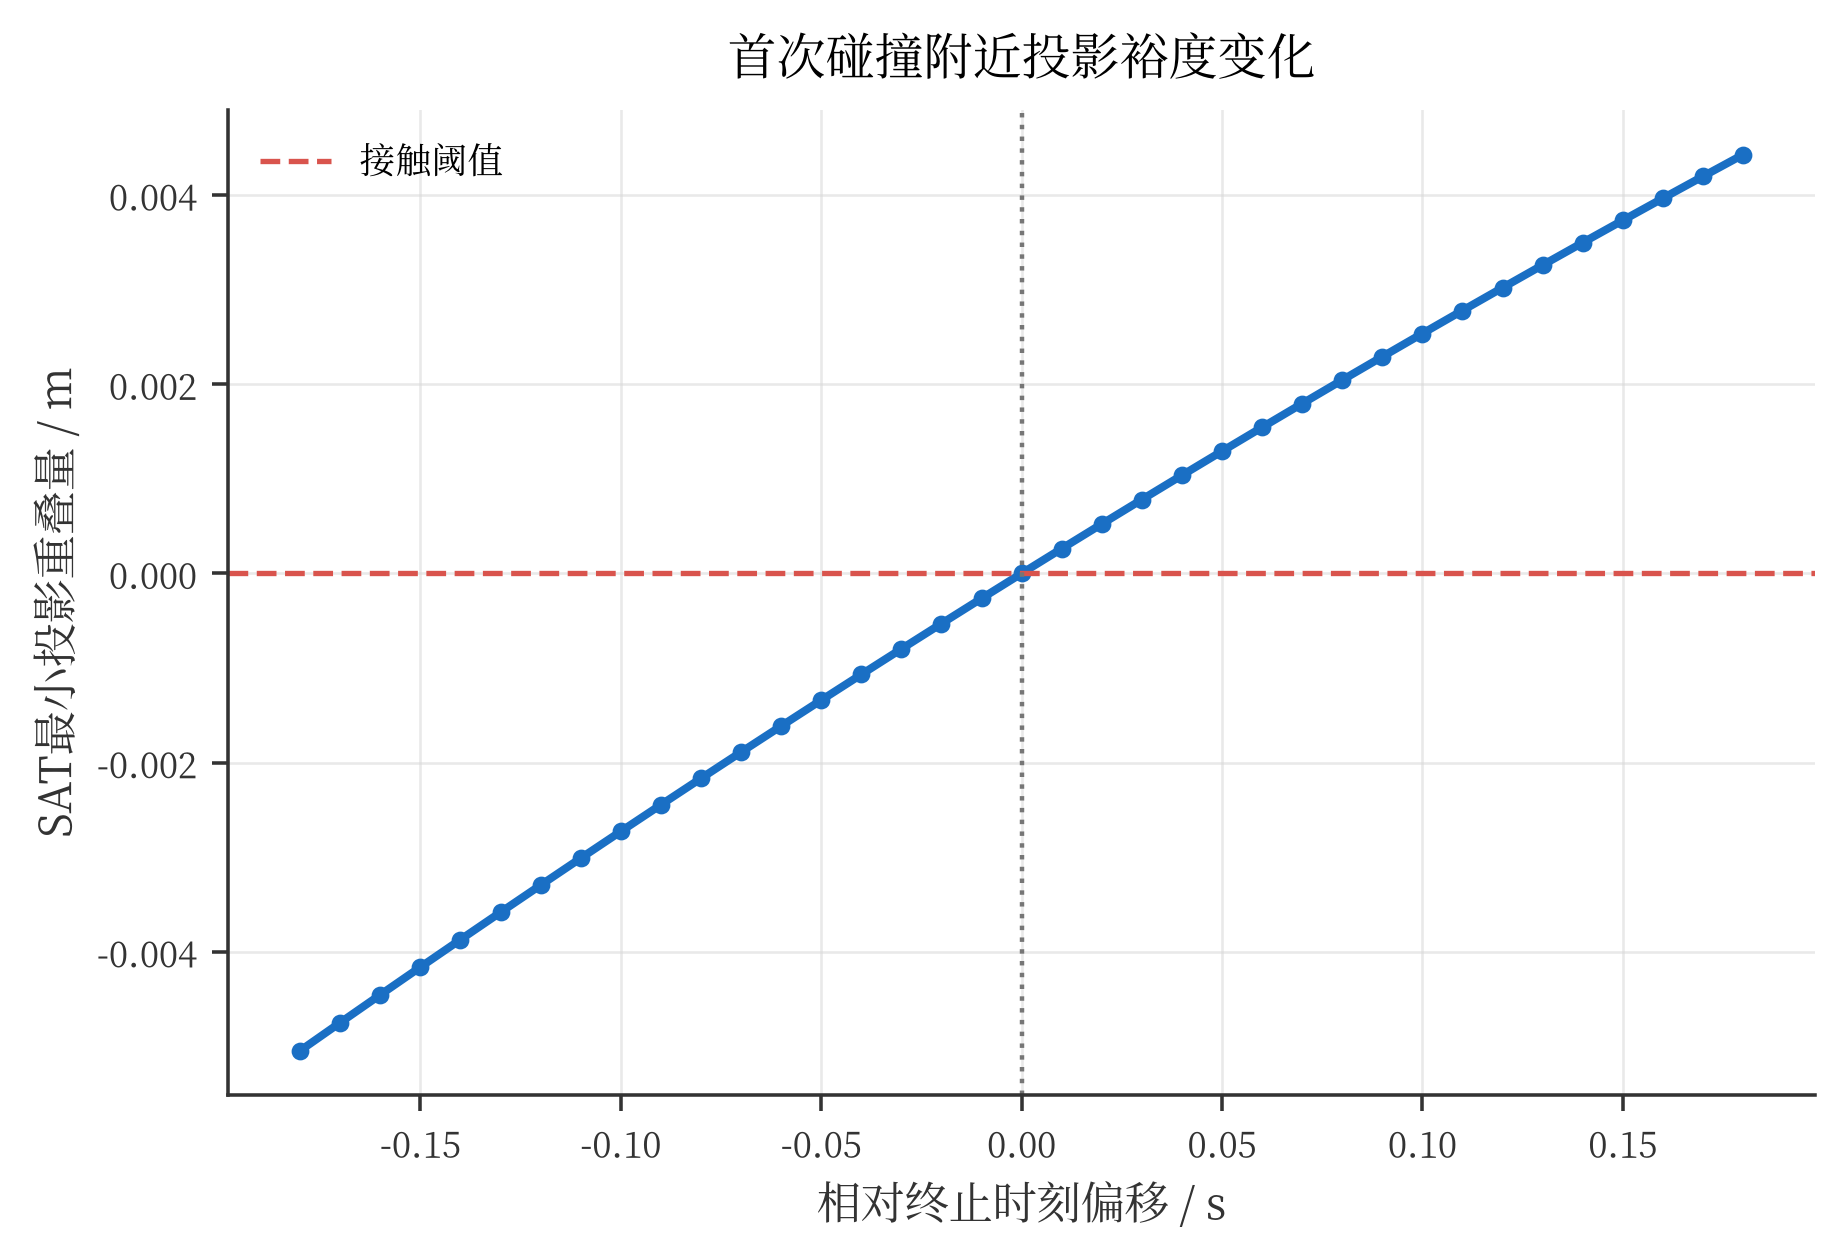
\includegraphics[width=0.88\textwidth]{figures/python/q2_collision_margin_trace.png}
\caption{首次碰撞附近最小投影裕度变化}
\label{fig:q2-collision-margin-trace}
\end{figure}

首次碰撞附近板凳龙的整体位置示意图如下，用于标明龙头与第8节板凳的相对位置关系。

\begin{figure}[H]
\centering
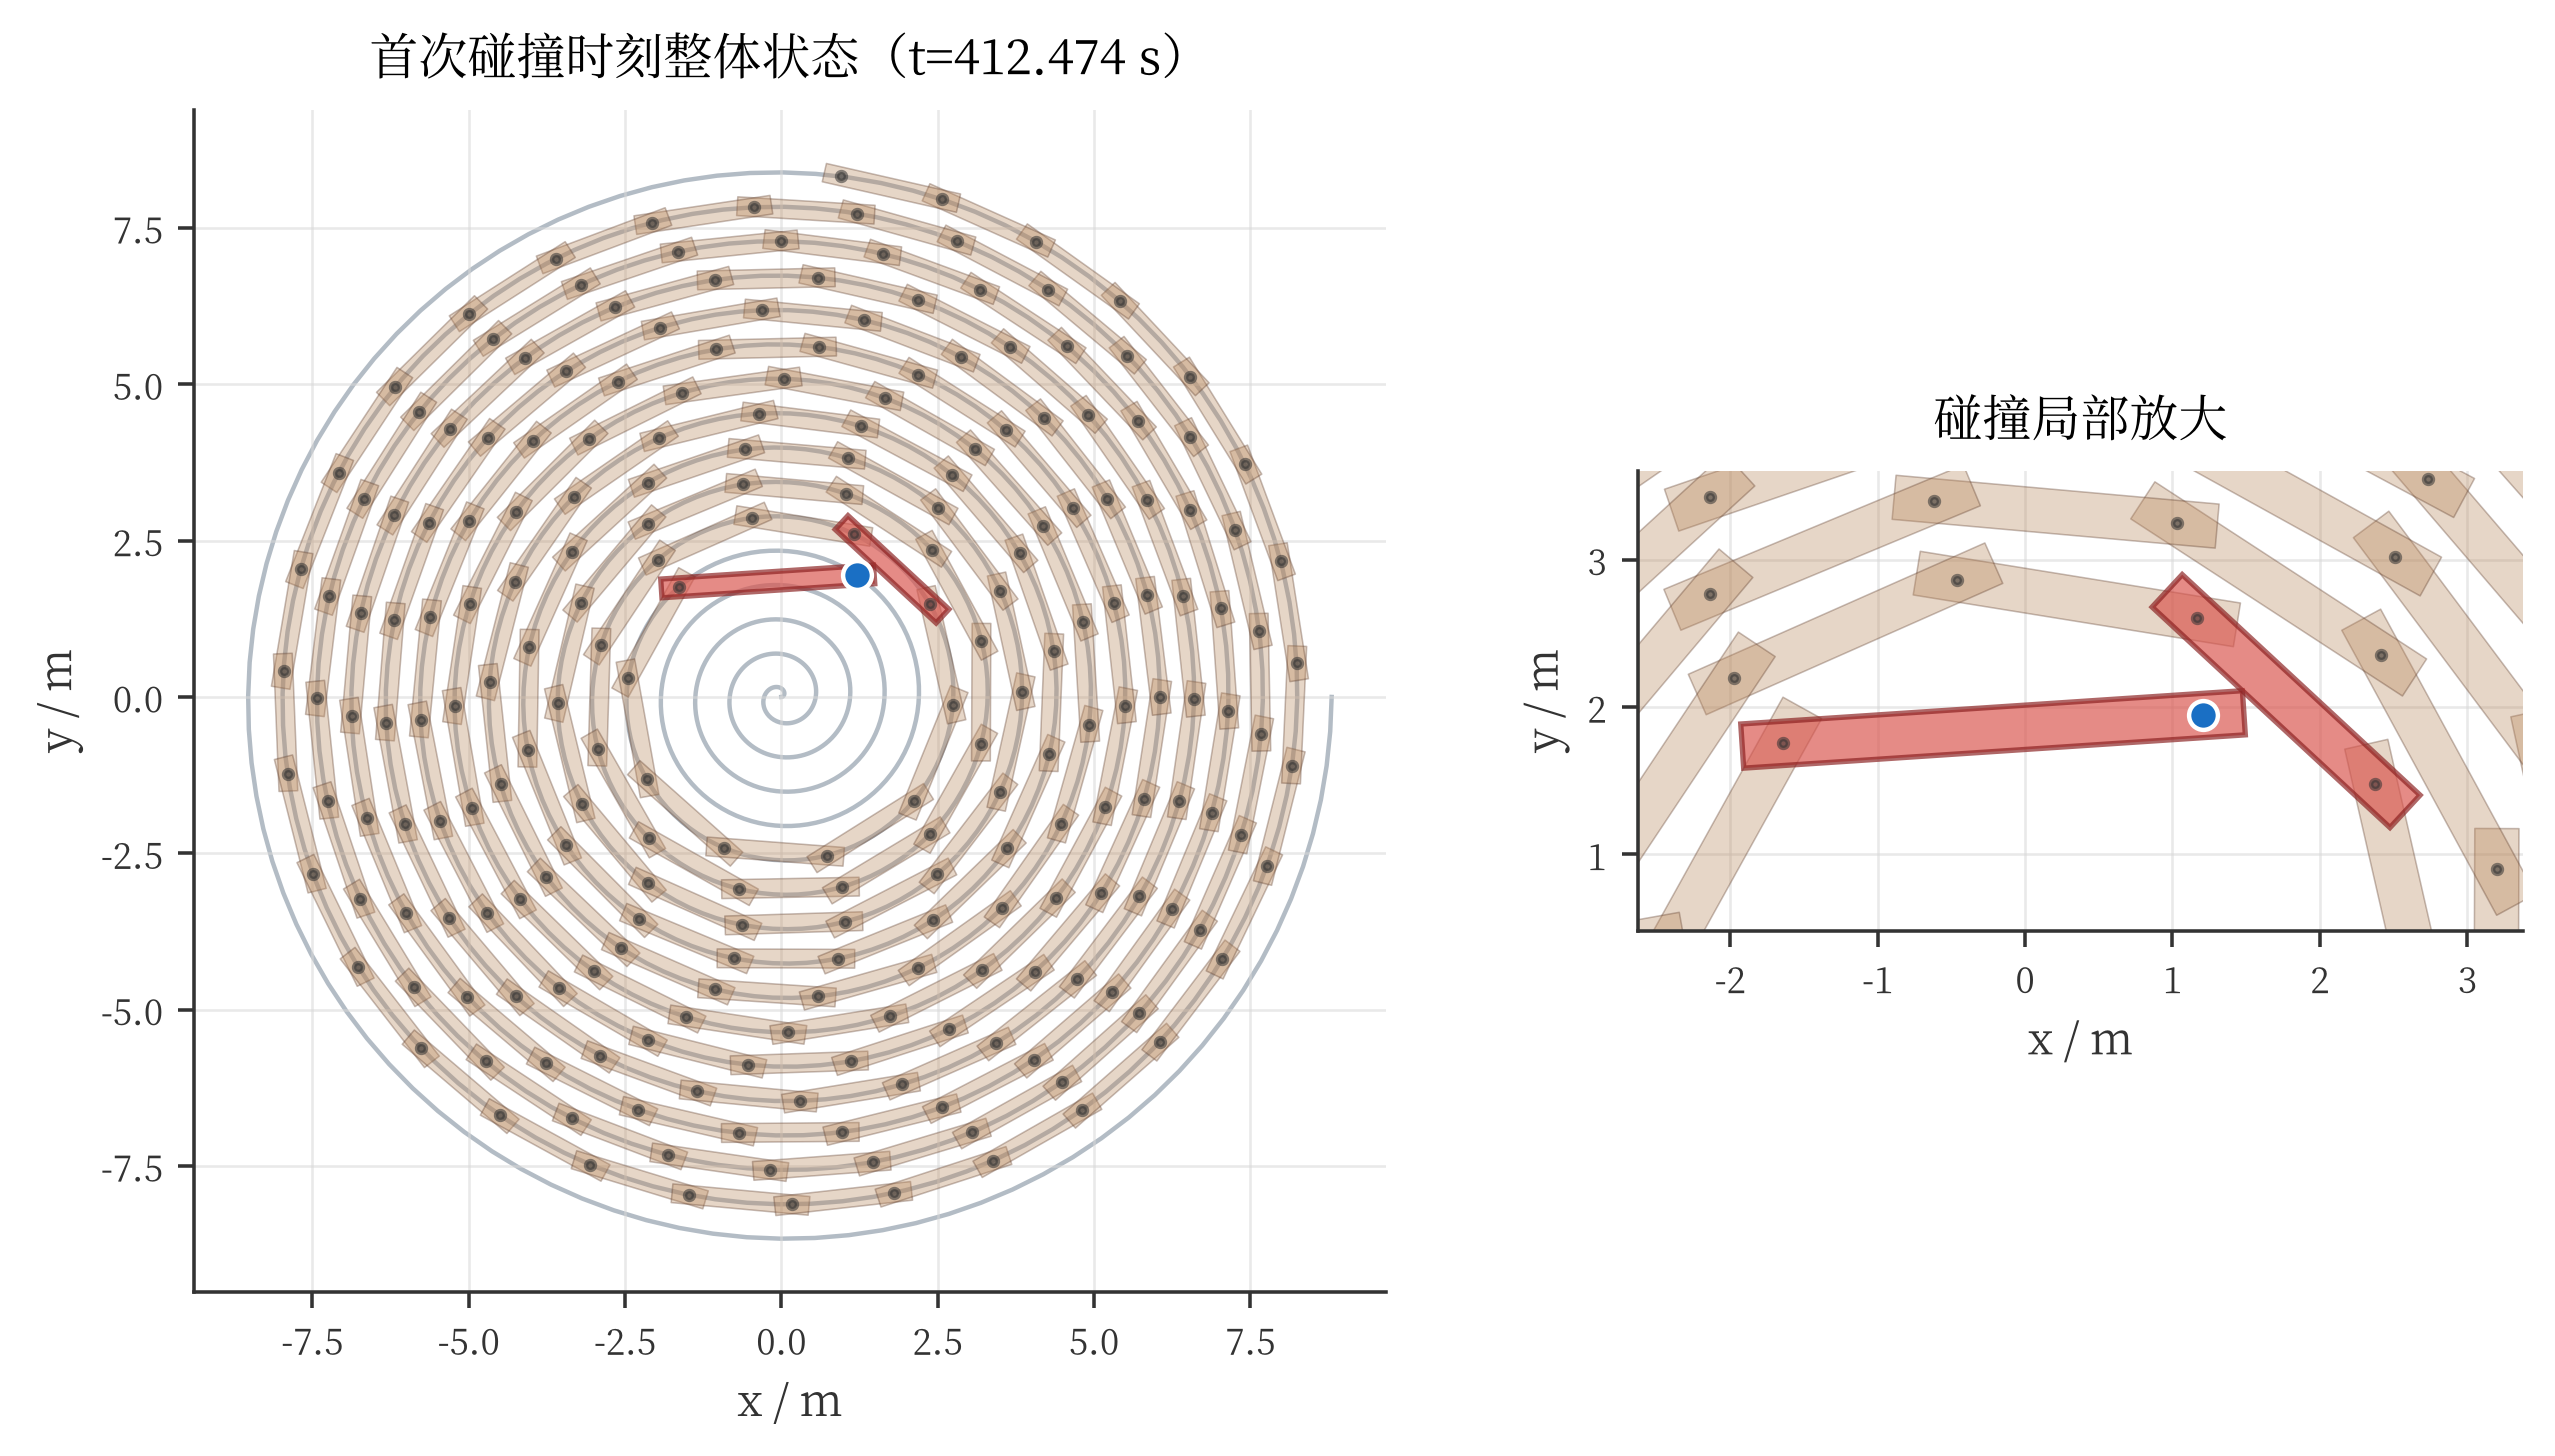
\includegraphics[width=0.92\textwidth]{figures/python/q2_collision_snapshot.png}
\caption{首次碰撞时刻附近板凳龙位置示意}
\label{fig:q2-collision-snapshot}
\end{figure}

终止状态已按附件二格式写入工作簿。该时刻全体把手速度范围为$0.973$到$1.000$ m/s。

\begin{table}[H]
\centering
\caption{问题二终止状态抽样表}
\label{tab:q2-terminal}
\begin{tabularx}{\textwidth}{lCCC}
\toprule
项目 & $x$ (m) & $y$ (m) & 速度 (m/s)\\
\midrule
龙头 & 1.209931 & 1.942784 & 1.000000\\
第1节龙身 & -1.643792 & 1.753399 & 0.991551\\
第51节龙身 & 1.281201 & 4.326588 & 0.976858\\
第101节龙身 & -0.536246 & -5.880138 & 0.974550\\
第151节龙身 & 0.968840 & -6.957479 & 0.973608\\
第201节龙身 & -7.893161 & -1.230764 & 0.973096\\
龙尾（后） & 0.956217 & 8.322736 & 0.972938\\
\bottomrule
\end{tabularx}
\end{table}

\subsection{小结}
问题二的终止时刻求解可以概括为“定义碰撞判定函数$\chi(t)$，定位其由0跃迁到1的临界点”。分离轴原理提供了矩形相交判定的数学基础，扫描与二分则提供了临界时刻的数值定位方式。该处理方式比仅凭中心线或经验距离判断更符合题目的实体碰撞要求。

\section{问题三：最小螺距的确定}
\subsection{建模思路}
问题三要求确定龙头前把手能够盘入半径为4.5 m的调头空间边界时所需的最小螺距。螺距越小，相邻圈螺线越密，龙头附近的板凳越容易与外圈板凳接近。因此，我们先以题目给定的55 cm作为初始螺距，并逐步减小螺距进行分析。

当螺距为55 cm时，根据前两问的计算过程，舞龙队在到达调头空间边界之前仍具有较大的空间余量。因此，最小螺距必然不大于55 cm。接下来从该上界出发，按步长逐步缩小螺距；每给定一个螺距，就判断龙头前把手从初始位置盘入到调头空间边界的过程中是否出现接触风险。若没有出现接触风险，则继续减小螺距；若出现接触风险，则退回上一螺距，并缩小步长继续搜索，直到步长达到给定精度。

\subsection{建立模型}
沿用问题一中的等距螺线模型，设螺距为 \(d\)，则盘入螺线可表示为
\[
r(\theta)=\frac{d}{2\pi}\theta,\qquad
x(\theta)=r(\theta)\cos\theta,\qquad
y(\theta)=r(\theta)\sin\theta.
\]
当龙头前把手到达调头空间边界时，有
\[
r(\theta_0)=R,\qquad R=4.5\ \text{m},
\]
即
\[
\theta_0(d)=\frac{2\pi R}{d}.
\]

龙头前把手到达调头空间边界时的几何关系示意图如下。图中边界圆与盘入螺线的交点对应$\theta_0(d)$，也是本问判断“能否盘入调头空间”的终点状态。

\begin{figure}[H]
\centering
\placeholderimage{5.4cm}{
图位预留：龙头到达调头边界示意图。\\[0.4em]
图中标出半径$R=4.5$ m的调头圆、盘入螺线$r=d\theta/(2\pi)$、\\
边界交点以及龙头前把手到达边界时的参数$\theta_0(d)$。
}
\caption{龙头前把手到达调头空间边界的几何示意}
\label{fig:q3-boundary}
\end{figure}

对于给定的 \(\theta\) 与 \(d\)，由相邻把手距离递推得到前若干把手坐标
\[
P_k(\theta,d)=\bigl(x_k(\theta,d),y_k(\theta,d)\bigr),\qquad k=0,1,\ldots,35.
\]
其中，龙头板凳的把手间距取 \(\ell_H=2.86\) m，其余板凳的把手间距取 \(\ell_B=1.65\) m。递推时通过
\[
\|P_{k+1}(\theta,d)-P_k(\theta,d)\|_2=\ell_k
\]
确定下一把手对应的角参数。

在临界碰撞判断中，主要考察龙头及其后一节板凳与前方若干龙身板凳之间的相对位置。对第 \(j\) 块板凳，其中心轴线由相邻把手 \(P_j,P_{j+1}\) 确定，记为
\[
A_jx+B_jy+C_j=0,
\]
其中
\[
A_j=y_{j+1}-y_j,\qquad
B_j=x_j-x_{j+1},\qquad
C_j=-x_jy_{j+1}+x_{j+1}y_j.
\]

龙头和第1节龙身的外侧角点由把手连线方向、法向方向以及板凳宽度确定。设这些角点构成集合 \(\mathcal{V}(\theta,d)\)，角点 \(V=(x_V,y_V)\) 到第 \(j\) 块板凳轴线的距离为
\[
\rho(V,L_j)=
\frac{|A_jx_V+B_jy_V+C_j|}
{\sqrt{A_j^2+B_j^2}}.
\]
取 \(j=3,\ldots,30\) 作为待检板凳范围，定义
\[
D(\theta,d)=
\min_{\substack{V\in\mathcal{V}(\theta,d)\\3\le j\le 30}}
\rho(V,L_j).
\]

由于板凳宽度为0.30 m，半宽为0.15 m。当龙头附近外侧角点到其他板凳轴线的最小距离降至0.15 m时，可认为实体轮廓到达接触临界。因此，判定函数为
\[
F(d)=\min_{\theta\in[\theta_0(d),\,\theta_0(d)+6]}D(\theta,d)-0.15.
\]
若 \(F(d)>0\)，说明在该螺距下未达到接触临界；若 \(F(d)\le 0\)，说明该螺距下已经出现接触风险。

\subsection{搜索最小螺距}
为了搜索最小螺距，我们采用逐步逼近的方法。

\textbf{Step1：确定初始螺距。} 取题设螺距 \(d=0.55\) m作为初始值，并选取0.01 m作为初始步长。

\textbf{Step2：判断是否发生碰撞。} 对当前螺距，计算龙头到达调头空间边界时的 \(\theta_0(d)\)，并在 \([\theta_0(d),\theta_0(d)+6]\) 内检查龙头及第1节龙身与第3至第30节龙身之间的距离关系。

\textbf{Step3：循环迭代。} 若未达到接触临界，则继续减小螺距；若达到接触临界，则返回上一螺距，并将步长缩小为原来的十分之一，继续判断。

\textbf{Step4：终止。} 当步长缩小到 \(10^{-6}\) m时停止循环，得到较为精确的最小螺距。

根据上述过程，得到不同搜索步长下的最小螺距近似值，如表\ref{tab:q3-result}所示。

\begin{table}[H]
\centering
\caption{逐步逼近最小螺距}
\label{tab:q3-result}
\begin{tabularx}{0.82\textwidth}{CCC}
\toprule
步长 & 螺距 & 单位\\
\midrule
0.01 & 0.46 & m\\
0.001 & 0.451 & m\\
0.0001 & 0.4504 & m\\
0.00001 & 0.45034 & m\\
0.000001 & 0.450332 & m\\
\bottomrule
\end{tabularx}
\end{table}

保留两位小数后，盘入调头空间所需的最小螺距为
\[
d_{\min}=0.45\ \text{m}.
\]
在粗搜索阶段，螺距 \(d=0.45\) m 已触发接触风险，这说明最小可行螺距位于0.45 m的右侧；继续细化后得到上述结果。

\section{问题四：调头路径的分段建模与状态递推}
\subsection{问题分解}
问题四给出盘入螺距为1.7 m，要求在半径4.5 m的调头空间内构造盘入与盘出之间的连接路径，并输出$-100$到$100$ s的运动状态。本问先由螺线与调头圆的交点确定调头入点，再按两段相切圆弧和半径比$2:1$建立调头路径，最后在该复合路径上递推全队把手状态。

\subsection{调头曲线的几何关系}
设盘入螺线与盘出螺线关于调头空间中心对称，中间连接段由两段相切圆弧组成，且满足
\[
R_1=2R_2.
\]
为便于表达，设盘入螺线与圆弧1的切点为$P_{\mathrm{in}}$，两圆弧切点为$Q$，圆弧2与盘出螺线切点为$P_{\mathrm{out}}$。那么整条路径由四段拼接而成：
\[
\text{盘入螺线}\to \text{圆弧1}\to \text{圆弧2}\to \text{盘出螺线}.
\]

为了使曲线连续且光滑，相邻段在连接点处应满足位置连续与切向连续。记盘入段与盘出段在边界处的切向单位向量分别为$\bm t_{\mathrm{in}}$和$\bm t_{\mathrm{out}}$，则圆弧1、圆弧2的圆心分别落在对应切点的法线方向上；再结合两圆弧相切与半径比约束，可确定圆心、半径和圆弧转角。

\subsection{固定交点下的几何关系证明}
设盘入螺距为$p=1.7$ m，令
\[
b=\frac{p}{2\pi},\qquad r=b\theta.
\]
调头空间为圆域
\[
\Omega=\{(x,y):x^2+y^2\le R^2\},\qquad R=4.5\ \text{m}.
\]
盘入螺线第一次到达调头圆边界时满足
\[
r(\theta_F)=R,
\]
由此得到入点对应的极角
\[
\theta_F=\frac{R}{b}=\frac{2\pi R}{p}.
\]
对应的交点为
\[
F=P_{\mathrm{in}}=
\bigl(R\cos\theta_F,\ R\sin\theta_F\bigr).
\]
盘出螺线与盘入螺线关于调头空间中心成中心对称，因此出点为
\[
P_{\mathrm{out}}=-P_{\mathrm{in}}.
\]
固定交点情形下的调头曲线几何关系示意图如下。

\begin{figure}[H]
\centering
\placeholderimage{6.2cm}{
图位预留：固定交点调头曲线几何示意图。\\[0.4em]
图中标出调头圆$x^2+y^2=R^2$、盘入螺线$r=b\theta$、盘出螺线的中心对称曲线、\\
交点$F=P_{\mathrm{in}}$、对称点$P_{\mathrm{out}}$、切向量$\bm t_{\mathrm{in}},\bm t_{\mathrm{out}}$、\\
两段相切圆弧的圆心$C_1,C_2$以及圆弧连接点$Q$。
}
\caption{固定交点情形下调头路径的几何关系示意}
\label{fig:q4-fixed-intersection}
\end{figure}

由螺线参数方程
\[
P(\theta)=b\theta(\cos\theta,\sin\theta)
\]
可得切向量
\[
P'(\theta)=b(\cos\theta-\theta\sin\theta,\ \sin\theta+\theta\cos\theta).
\]
于是盘入端点的单位切向量为
\[
\bm t_{\mathrm{in}}=
\frac{P'(\theta_F)}{\|P'(\theta_F)\|}.
\]
记径向单位向量为
\[
\bm e_r=(\cos\theta_F,\sin\theta_F).
\]
设螺线切线与调头圆切线之间的夹角为$\alpha$，则
\[
\alpha=\frac{\pi}{2}-\arccos(\bm t_{\mathrm{in}}\cdot\bm e_r).
\]
将$\bm t_{\mathrm{in}}$代入上式，可得
\[
\alpha
=\frac{\pi}{2}
-\arccos
\frac{(\cos\theta_F-\theta_F\sin\theta_F)\cos\theta_F
+(\sin\theta_F+\theta_F\cos\theta_F)\sin\theta_F}
{\sqrt{\theta_F^2+1}}
=\frac{\pi}{2}-\arccos\frac{1}{\sqrt{\theta_F^2+1}}.
\]
两段圆弧与盘入、盘出螺线相切，且两段圆弧在连接点$Q$处相切。由图\ref{fig:q4-fixed-intersection}中的直角三角关系，圆心连线对应的有效半径和为
\[
R_1+R_2=\frac{R}{\cos\alpha}.
\]
又由题设
\[
R_1=2R_2,
\]
解得
\[
R_1=\frac{2R}{3\cos\alpha},\qquad
R_2=\frac{R}{3\cos\alpha}.
\]
连接点$Q$两侧的圆弧转角相同，均为
\[
\beta=\pi-2\alpha.
\]
于是调头曲线长度为
\[
L_{\mathrm{turn}}
=R_1\beta+R_2\beta
=(R_1+R_2)(\pi-2\alpha)
=\frac{R}{\cos\alpha}(\pi-2\alpha).
\]
其中
\[
\theta_F=\frac{2\pi R}{p},\qquad
\alpha=\frac{\pi}{2}-\arccos\frac{1}{\sqrt{\theta_F^2+1}}.
\]
代入$p=1.7$ m、$R=4.5$ m，得到
\[
\theta_F=16.631961,\quad
\alpha=0.060053,
\]
\[
R_1=3.005418\ \text{m},\quad
R_2=1.502709\ \text{m},
\]
\[
L_{\mathrm{turn}}=13.621245\ \text{m}.
\]

\subsection{路径参数与求解流程}
根据上述几何关系，调头路径满足
\[
\begin{cases}
\text{圆弧1与盘入螺线相切},\\
\text{圆弧1与圆弧2相切},\\
\text{圆弧2与盘出螺线相切},\\
R_1=2R_2,\\
P_{\mathrm{out}}=-P_{\mathrm{in}},\\
P_{\mathrm{in}}=(R\cos\theta_F,R\sin\theta_F).
\end{cases}
\]
求解时先计算$\theta_F$和$\alpha$，再由半径比求$R_1,R_2$，最后按盘入螺线、圆弧1、圆弧2、盘出螺线的顺序建立弧长参数函数。

\begin{algorithm}[H]
\caption{问题四固定交点调头路径与状态求解流程}
\label{alg:q4-turn}
\textbf{Input:} 螺距$p=1.7$，调头空间半径$R=4.5$，整数时刻$t\in[-100,100]$。\\
\textbf{Output:} 调头路径参数、各时刻把手位置与速度。
\begin{enumerate}[label=\arabic*:, leftmargin=2.6em, itemsep=0.2em]
\item 计算盘入螺线与调头圆交点对应的极角$\theta_F=2\pi R/p$。
\item 由交点处螺线切向确定边界切线夹角$\alpha$。
\item 根据$R_1=2R/(3\cos\alpha)$和$R_2=R/(3\cos\alpha)$确定两段圆弧半径。
\item 按盘入螺线、圆弧1、圆弧2、中心对称盘出螺线的顺序建立复合弧长参数路径。
\item 对$t\in[-100,100]$逐秒递推全部把手位置，并由差分计算速度。
\item \textbf{return} 调头路径参数和全队运动状态。
\end{enumerate}
\end{algorithm}

按上述参数得到的调头路径整体示意图如下，用于展示盘入螺线、两段圆弧和盘出螺线的空间拼接关系。

\begin{figure}[H]
\centering
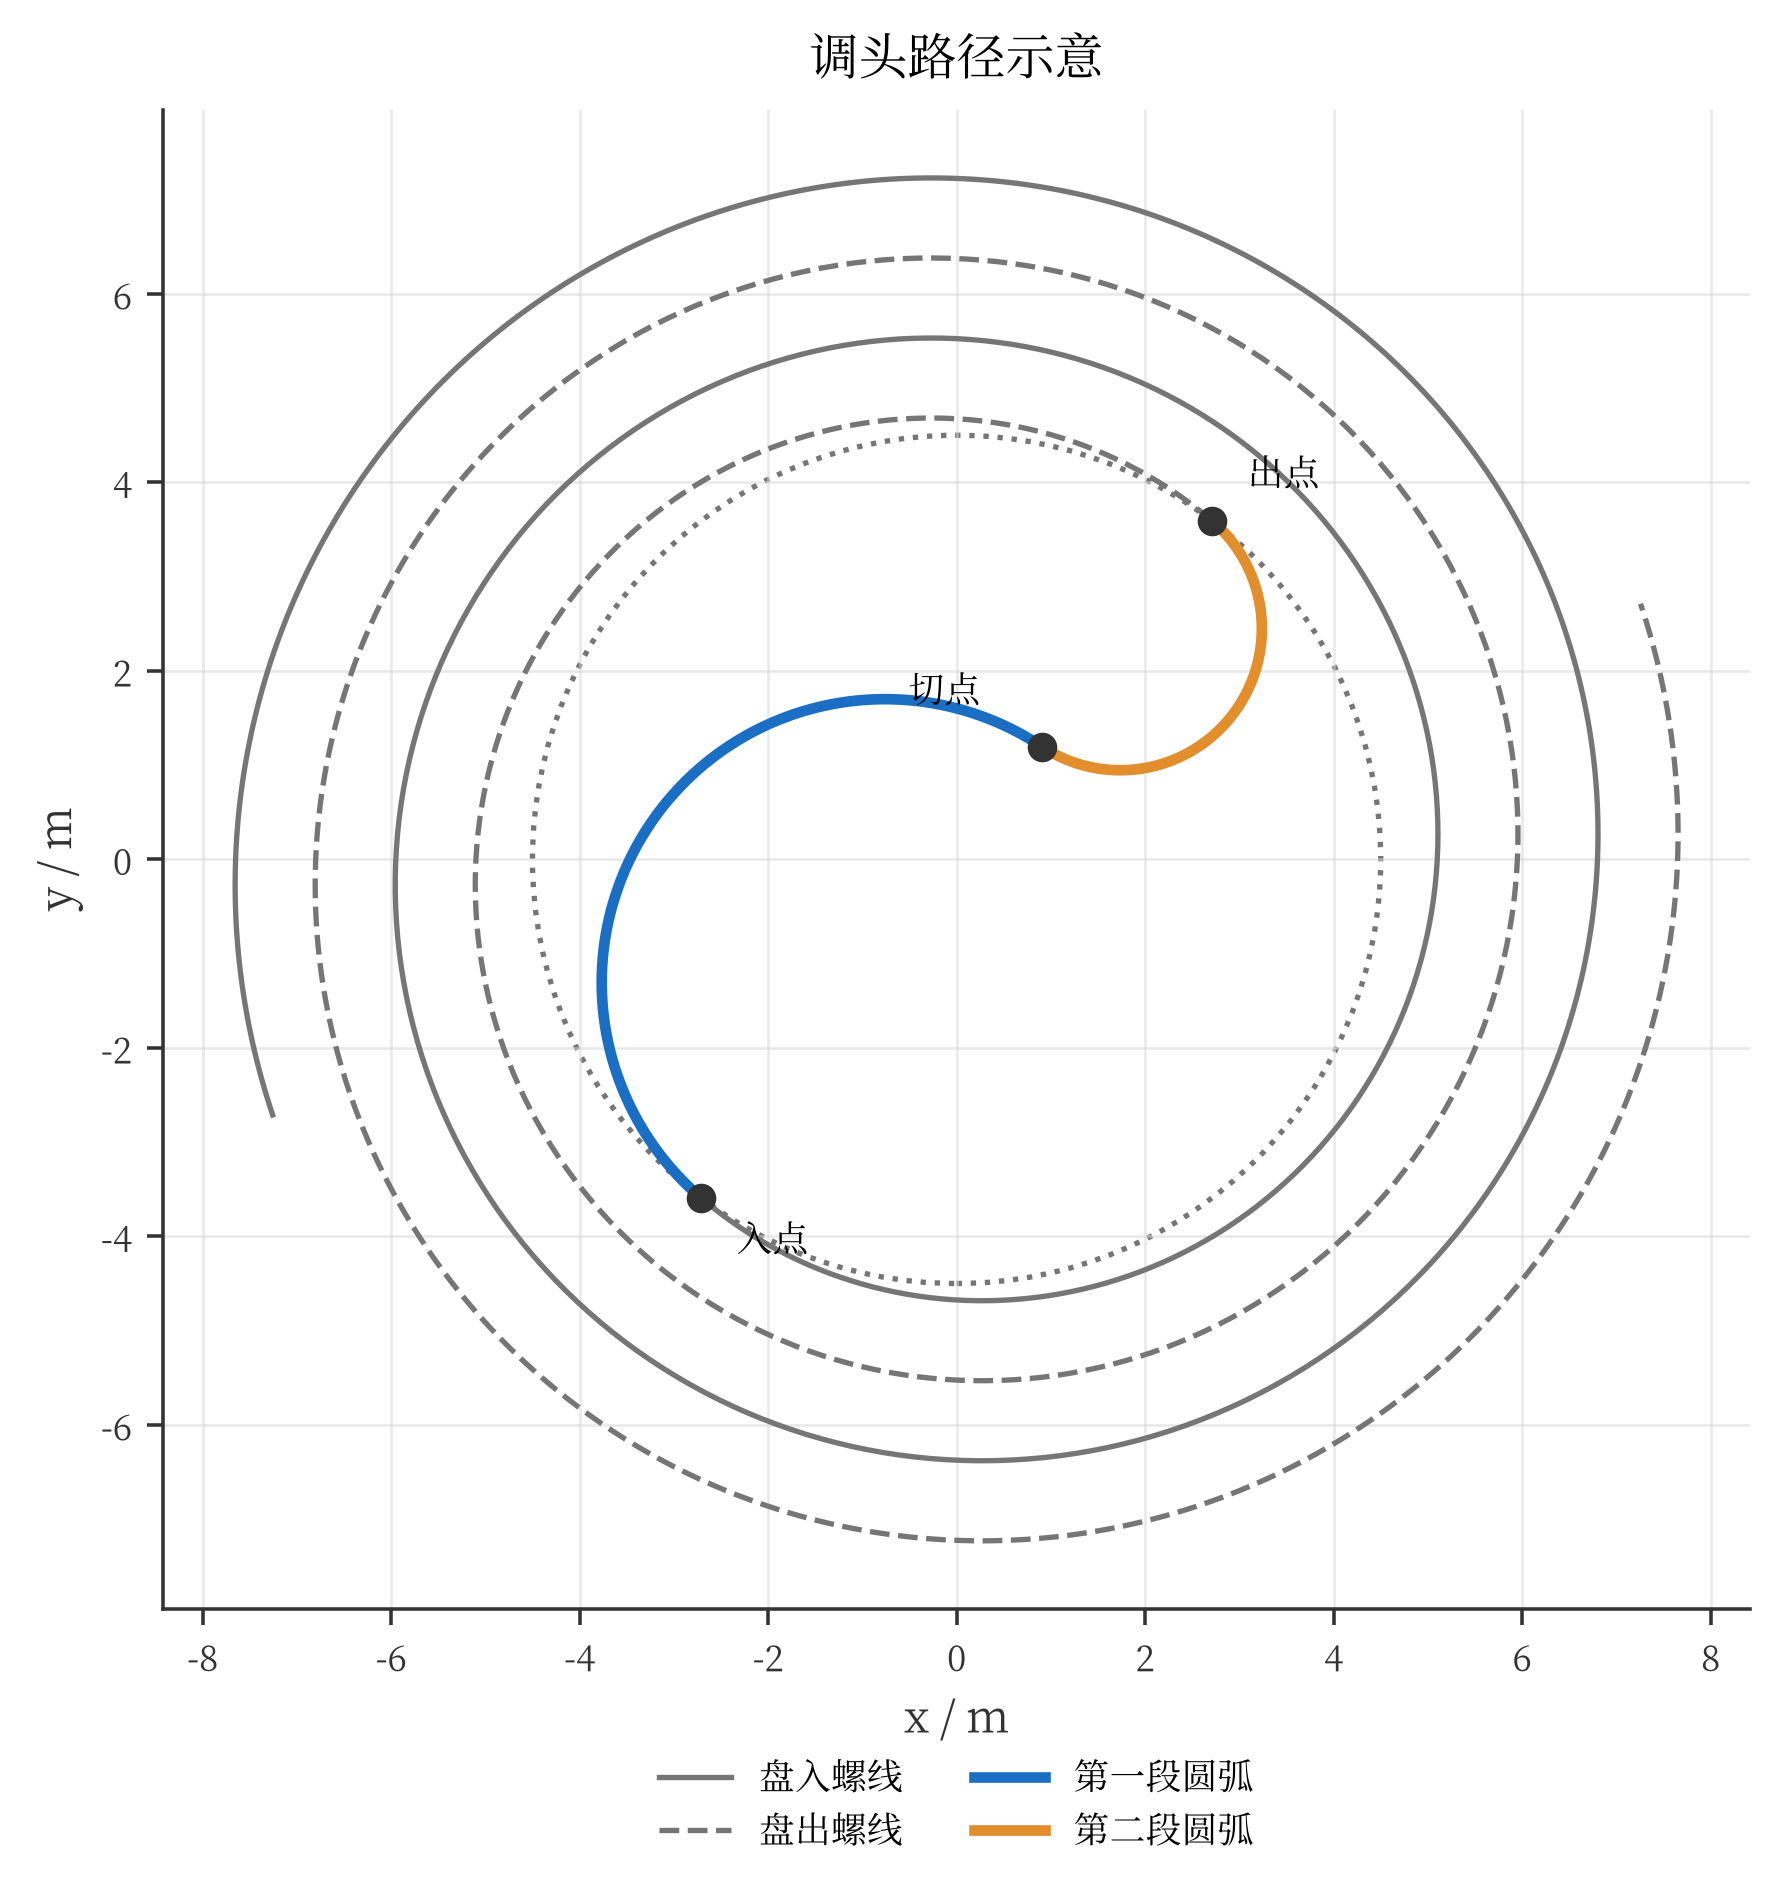
\includegraphics[width=0.92\textwidth]{figures/python/q4_turn_path_overview.png}
\caption{盘入、两段圆弧与盘出路径的整体示意}
\label{fig:q4-turn-path}
\end{figure}

\subsection{状态递推与结果}
在路径确定后，龙头前把手沿该复合路径以1 m/s运动。后续把手仍由固定把手间距逐节递推得到。对于任意时刻$t$，将路径视为弧长参数$s$的函数$P(s)$，先由头速确定龙头对应弧长，再由
\[
\|P_{i+1}(s)-P_i(s)\|_2=d_i
\]
逐节向后求解即可。速度采用问题一中的中心差分形式从位置序列计算。

调头路径参数如下：
\[
R_1=3.005418\ \text{m},\qquad
R_2=1.502709\ \text{m},
\]
\[
L_{\mathrm{turn}}=13.621245\ \text{m}.
\]
整段$-100$到$100$ s的运动状态按上述复合路径递推得到。完整位置表含224个把手在201个整数时刻的$x,y$坐标，规模为$449\times202$；完整速度表含224个把手在201个整数时刻的速度，规模为$225\times202$。两张表已写入结果工作簿\texttt{result4.xlsx}，表\ref{tab:q4-position-extract}和表\ref{tab:q4-speed-extract}列出关键把手在部分时刻的抽样结果。

板凳龙在盘入盘出复合路径上的整体状态示意图如下，用于展示路径改变后全队把手仍按固定距离逐节递推。

\begin{figure}[H]
\centering
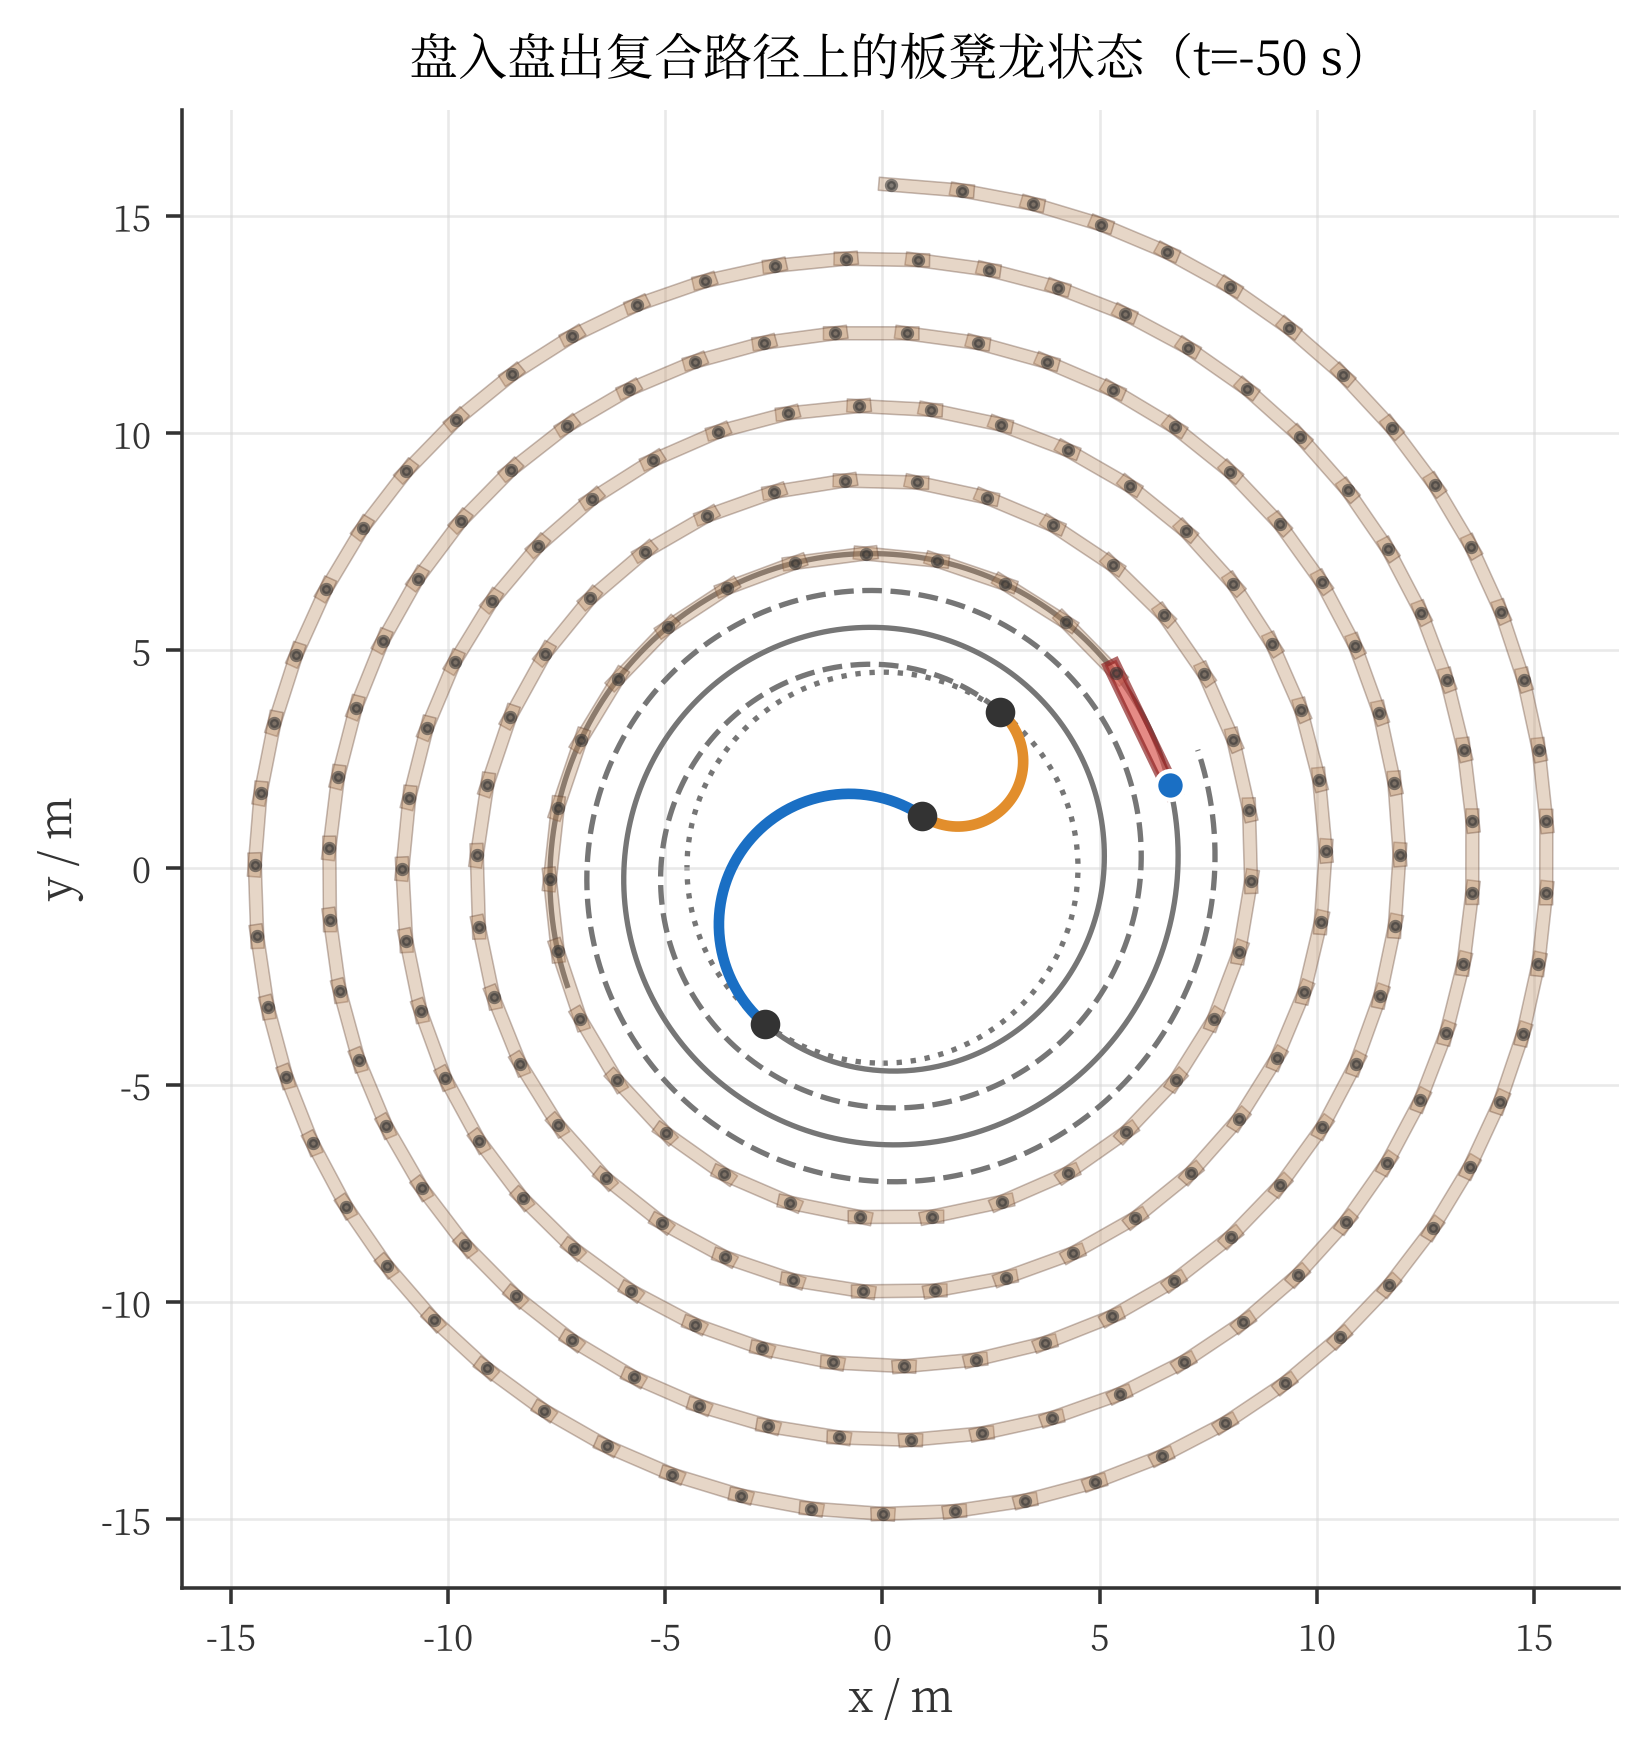
\includegraphics[width=0.92\textwidth]{figures/python/q4_composite_path_state.png}
\caption{板凳龙在盘入盘出复合路径上的状态示意}
\label{fig:q4-inout-snapshot}
\end{figure}

当龙头位于圆弧调头段时的板凳龙状态示意图如下，该图用于说明调头过程中仍采用同一套相邻把手距离递推约束。

\begin{figure}[H]
\centering
\placeholderimage{5.8cm}{
图位预留：板凳龙正在调头时的状态示意图。\\[0.4em]
图中突出显示龙头位于两段圆弧之一时的全队位置，\\
并标注圆弧段、盘入段、盘出段与调头空间边界。
}
\caption{板凳龙处于圆弧调头段时的状态示意}
\label{fig:q4-turning-snapshot}
\end{figure}

\begin{table}[H]
\centering
\caption{问题四调头路径参数表}
\label{tab:q4-result}
\begin{tabularx}{0.86\textwidth}{LCC}
\toprule
量 & 数值 & 单位\\
\midrule
入点极角$\theta_F$ & 16.631961 & rad\\
切线夹角$\alpha$ & 0.060053 & rad\\
圆弧1半径$R_1$ & 3.005418 & m\\
圆弧2半径$R_2$ & 1.502709 & m\\
圆弧转角$\beta$ & 3.021487 & rad\\
调头路径长度$L_{\mathrm{turn}}$ & 13.621245 & m\\
\bottomrule
\end{tabularx}
\end{table}

\begin{table}[H]
\centering
\caption{问题四关键把手位置抽样表}
\label{tab:q4-position-extract}
\begingroup
\setlength{\tabcolsep}{3pt}
\begin{tabularx}{\textwidth}{>{\raggedright\arraybackslash}p{0.15\textwidth}*{5}{R}}
\toprule
项目 & $-100$ s & $-50$ s & $0$ s & $50$ s & $100$ s\\
\midrule
龙头$x$ & 7.778034 & 6.608301 & -2.711856 & 1.332696 & -3.157229\\
龙头$y$ & 3.717164 & 1.898865 & -3.591078 & 6.175324 & 7.548511\\
第1节$x$ & 6.209273 & 5.366911 & -0.063534 & 3.862265 & -0.346890\\
第1节$y$ & 6.108521 & 4.475403 & -4.670888 & 4.840828 & 8.079166\\
第51节$x$ & -10.608038 & -3.629945 & 2.459962 & -1.671385 & 2.095033\\
第51节$y$ & 2.831491 & -8.963800 & -7.778145 & -6.076713 & 4.033787\\
第101节$x$ & -11.922761 & 10.125787 & 3.008493 & -7.591816 & -7.288774\\
第101节$y$ & -4.802378 & -5.972247 & 10.108539 & 5.175487 & 2.063875\\
第151节$x$ & -14.351032 & 12.974784 & -7.002789 & -4.605165 & 9.462513\\
第151节$y$ & -1.980993 & -3.810357 & 10.337482 & -10.386988 & -3.540357\\
第201节$x$ & -11.952942 & 10.522509 & -6.872842 & 0.336952 & 8.524374\\
第201节$y$ & 10.566998 & -10.807425 & 12.382609 & -13.177610 & 8.606933\\
龙尾$x$ & -1.011059 & 0.189809 & -1.933627 & 5.859094 & -10.980157\\
龙尾$y$ & -16.527573 & 15.720588 & -14.713128 & 12.612894 & -6.770006\\
\bottomrule
\end{tabularx}
\endgroup
\end{table}

\begin{table}[H]
\centering
\caption{问题四关键把手速度抽样表}
\label{tab:q4-speed-extract}
\begingroup
\setlength{\tabcolsep}{3pt}
\begin{tabularx}{\textwidth}{>{\raggedright\arraybackslash}p{0.18\textwidth}*{5}{R}}
\toprule
项目 & $-100$ s & $-50$ s & $0$ s & $50$ s & $100$ s\\
\midrule
龙头 & 1.000000 & 1.000000 & 1.000000 & 1.000000 & 1.000000\\
第1节龙身 & 0.999904 & 0.999762 & 0.998687 & 1.000363 & 1.000124\\
第51节龙身 & 0.999346 & 0.998642 & 0.995134 & 0.949935 & 1.003966\\
第101节龙身 & 0.999091 & 0.998248 & 0.994448 & 0.948482 & 1.096263\\
第151节龙身 & 0.998944 & 0.998047 & 0.994156 & 0.948038 & 1.095306\\
第201节龙身 & 0.998849 & 0.997925 & 0.993994 & 0.947823 & 1.094933\\
龙尾（后） & 0.998817 & 0.997885 & 0.993944 & 0.947760 & 1.094833\\
\bottomrule
\end{tabularx}
\endgroup
\end{table}

\subsection{小结}
Q4的核心是在固定交点、两段相切圆弧和半径比$2:1$的约束下建立复合路径，再以该路径为基础计算前后运动状态。该路径下相邻把手距离最大误差为$1.33\times10^{-9}$ m，说明逐节递推在调头前后仍保持了板凳连接约束。

\section{问题五：最大恒定速度的求解}
\subsection{模型建立}
问题五要求在问题四给定调头路径上，确定龙头前把手可采用的最大恒定速度，并保证任一把手速度均不超过2 m/s。与前四问不同，本问不再改变几何路径，而是在既定路径上讨论速度约束；因此核心是把全队速度响应转化为龙头速度的比例放大问题。

设单位头速下第$i$个把手在时刻$t$的速度为$v_i^{(1)}(t)$。当龙头恒定速度由1 m/s改为$v_H$时，路径形状和各把手间距约束不变，时间尺度按同一比例缩放，故各把手速度满足
\[
v_i(t;v_H)=v_H\,v_i^{(1)}(t),
\]
从而速度约束可写为
\[
\max_{i,t} v_i(t;v_H)\le 2.
\]
于是最大头速满足
\[
v_{\max}=\frac{2}{\max_{i,t} v_i^{(1)}(t)}.
\]
该式把“所有把手速度均受限”的多变量约束，化为单位头速下最大速度放大倍数的计算。后续只需先求出速度矩阵$\{v_i^{(1)}(t)\}$，再由其中的最大值反推龙头速度上界。

\subsection{速度递推与约束转化}
设第$i-1$个把手与第$i$个把手之间的连杆方向单位向量为$\bm e_i$，两把手所在路径处的切向单位向量分别为$\bm \tau_{i-1}$和$\bm \tau_i$。由相邻把手距离约束对时间求导，可得沿连杆方向的速度投影相等：
\[
v_{i-1}(\bm \tau_{i-1}\cdot \bm e_i)
=v_i(\bm \tau_i\cdot \bm e_i).
\]
因此，在单位龙头速度$v_0=1$ m/s下，可逐节递推
\[
v_i^{(1)}(t)
=v_{i-1}^{(1)}(t)
\left|
\frac{\bm \tau_{i-1}\cdot \bm e_i}
{\bm \tau_i\cdot \bm e_i}
\right|.
\]
对所有$i=0,1,\ldots,223$和$t=-100,-99,\ldots,100$ s计算$v_i^{(1)}(t)$，即可得到速度放大倍数
\[
\lambda_{\max}=\max_{i,t} v_i^{(1)}(t).
\]
为定位约束最紧的位置和时刻，进一步定义
\[
M(t)=\max_i v_i^{(1)}(t),\qquad
G_i=\max_t v_i^{(1)}(t).
\]
其中$M(t)$反映每一时刻全队速度上界的变化，$G_i$反映各把手在整个调头过程中的最大速度放大情况。前者用于定位限制时刻，后者用于解释限制把手来源。

基于$M(t)$可绘制全队最大把手速度随时间变化图，用于说明速度约束如何在调头过程中形成。

\begin{figure}[H]
\centering
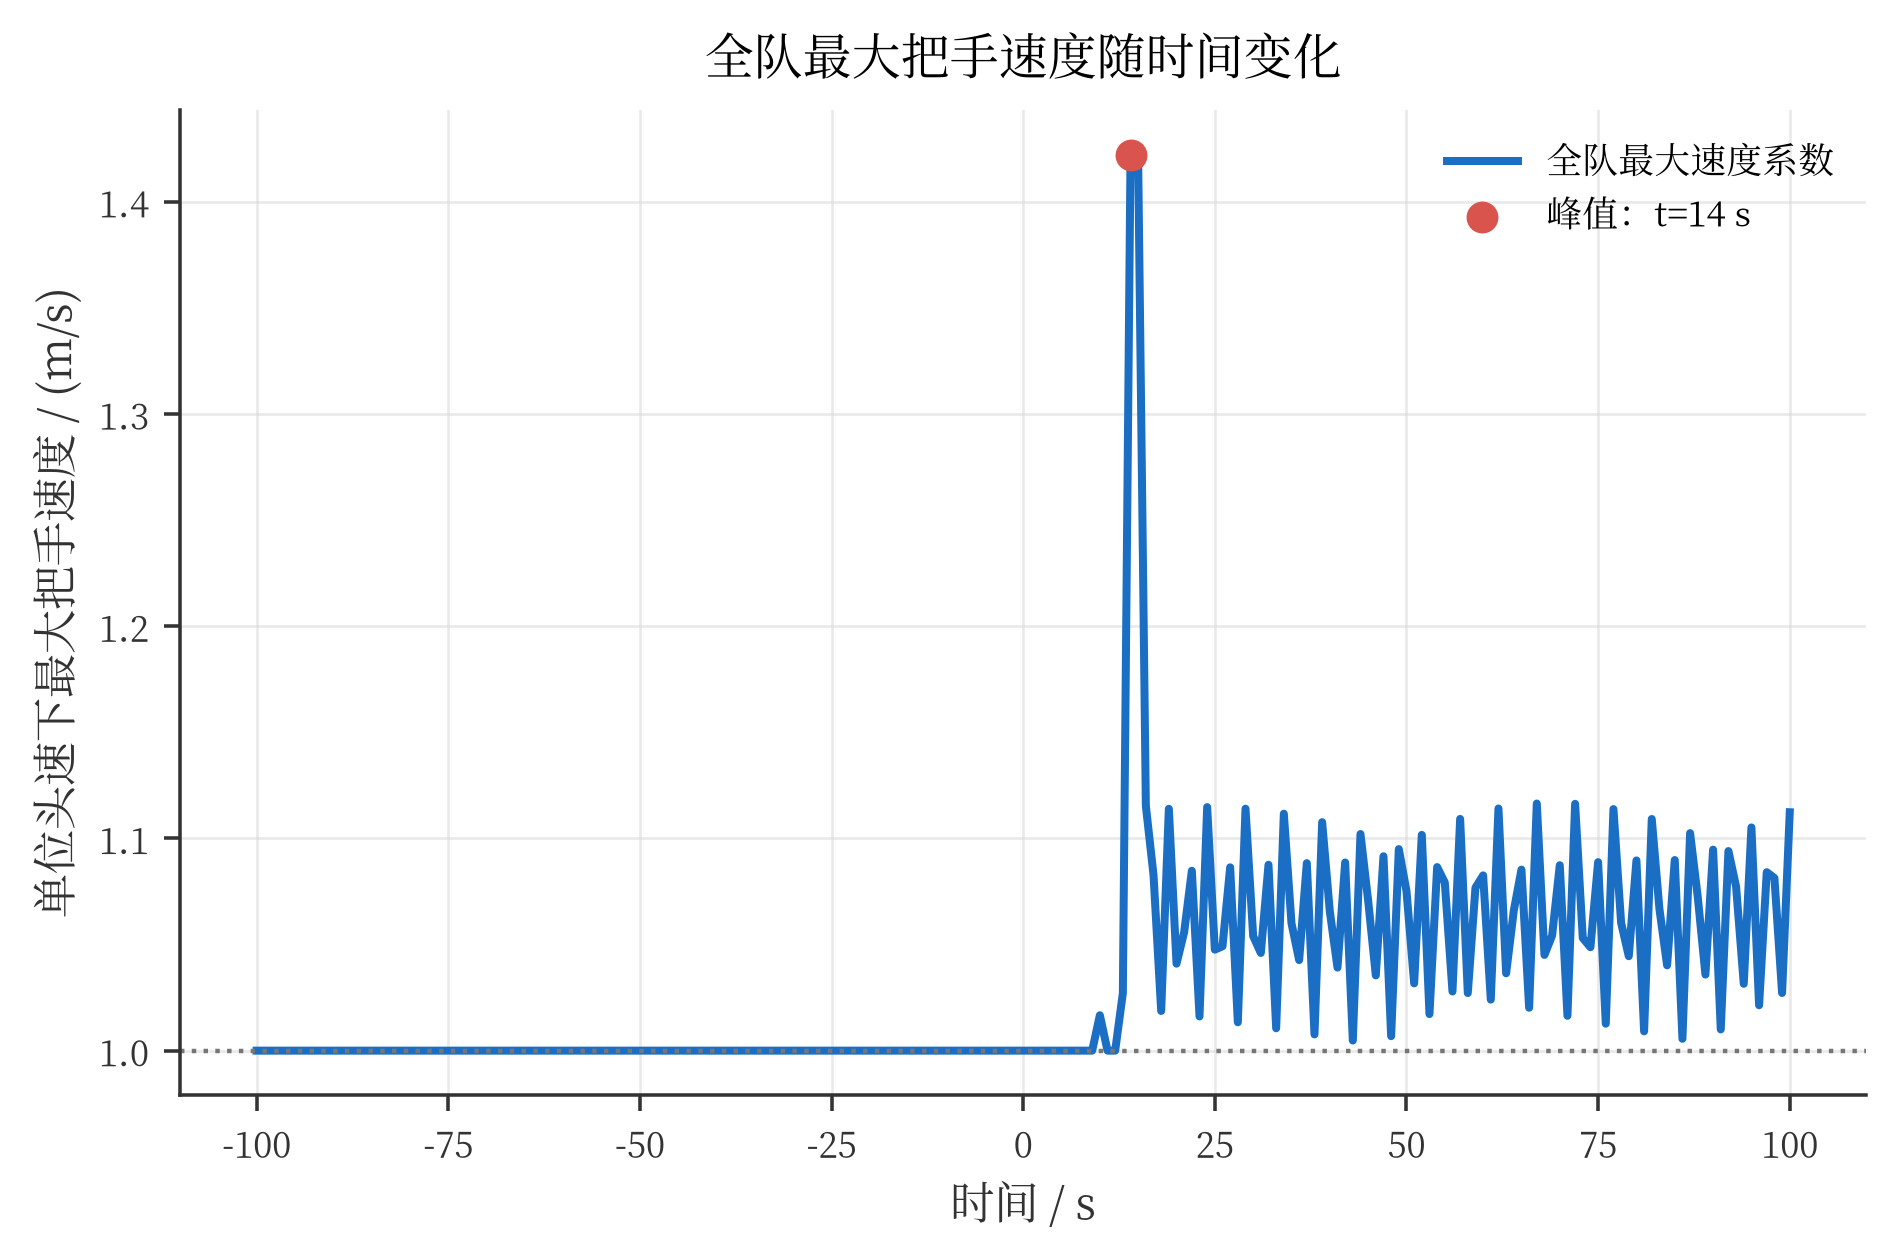
\includegraphics[width=0.88\textwidth]{figures/python/q5_time_max_speed.png}
\caption{单位头速下全队最大把手速度随时间变化}
\label{fig:q5-max-speed-time}
\end{figure}

进一步把速度放大倍数按“把手编号--时刻”展开，可得到单位头速下的速度放大倍数热力图，用于同时观察限制时刻与限制把手的位置。

\begin{figure}[H]
\centering
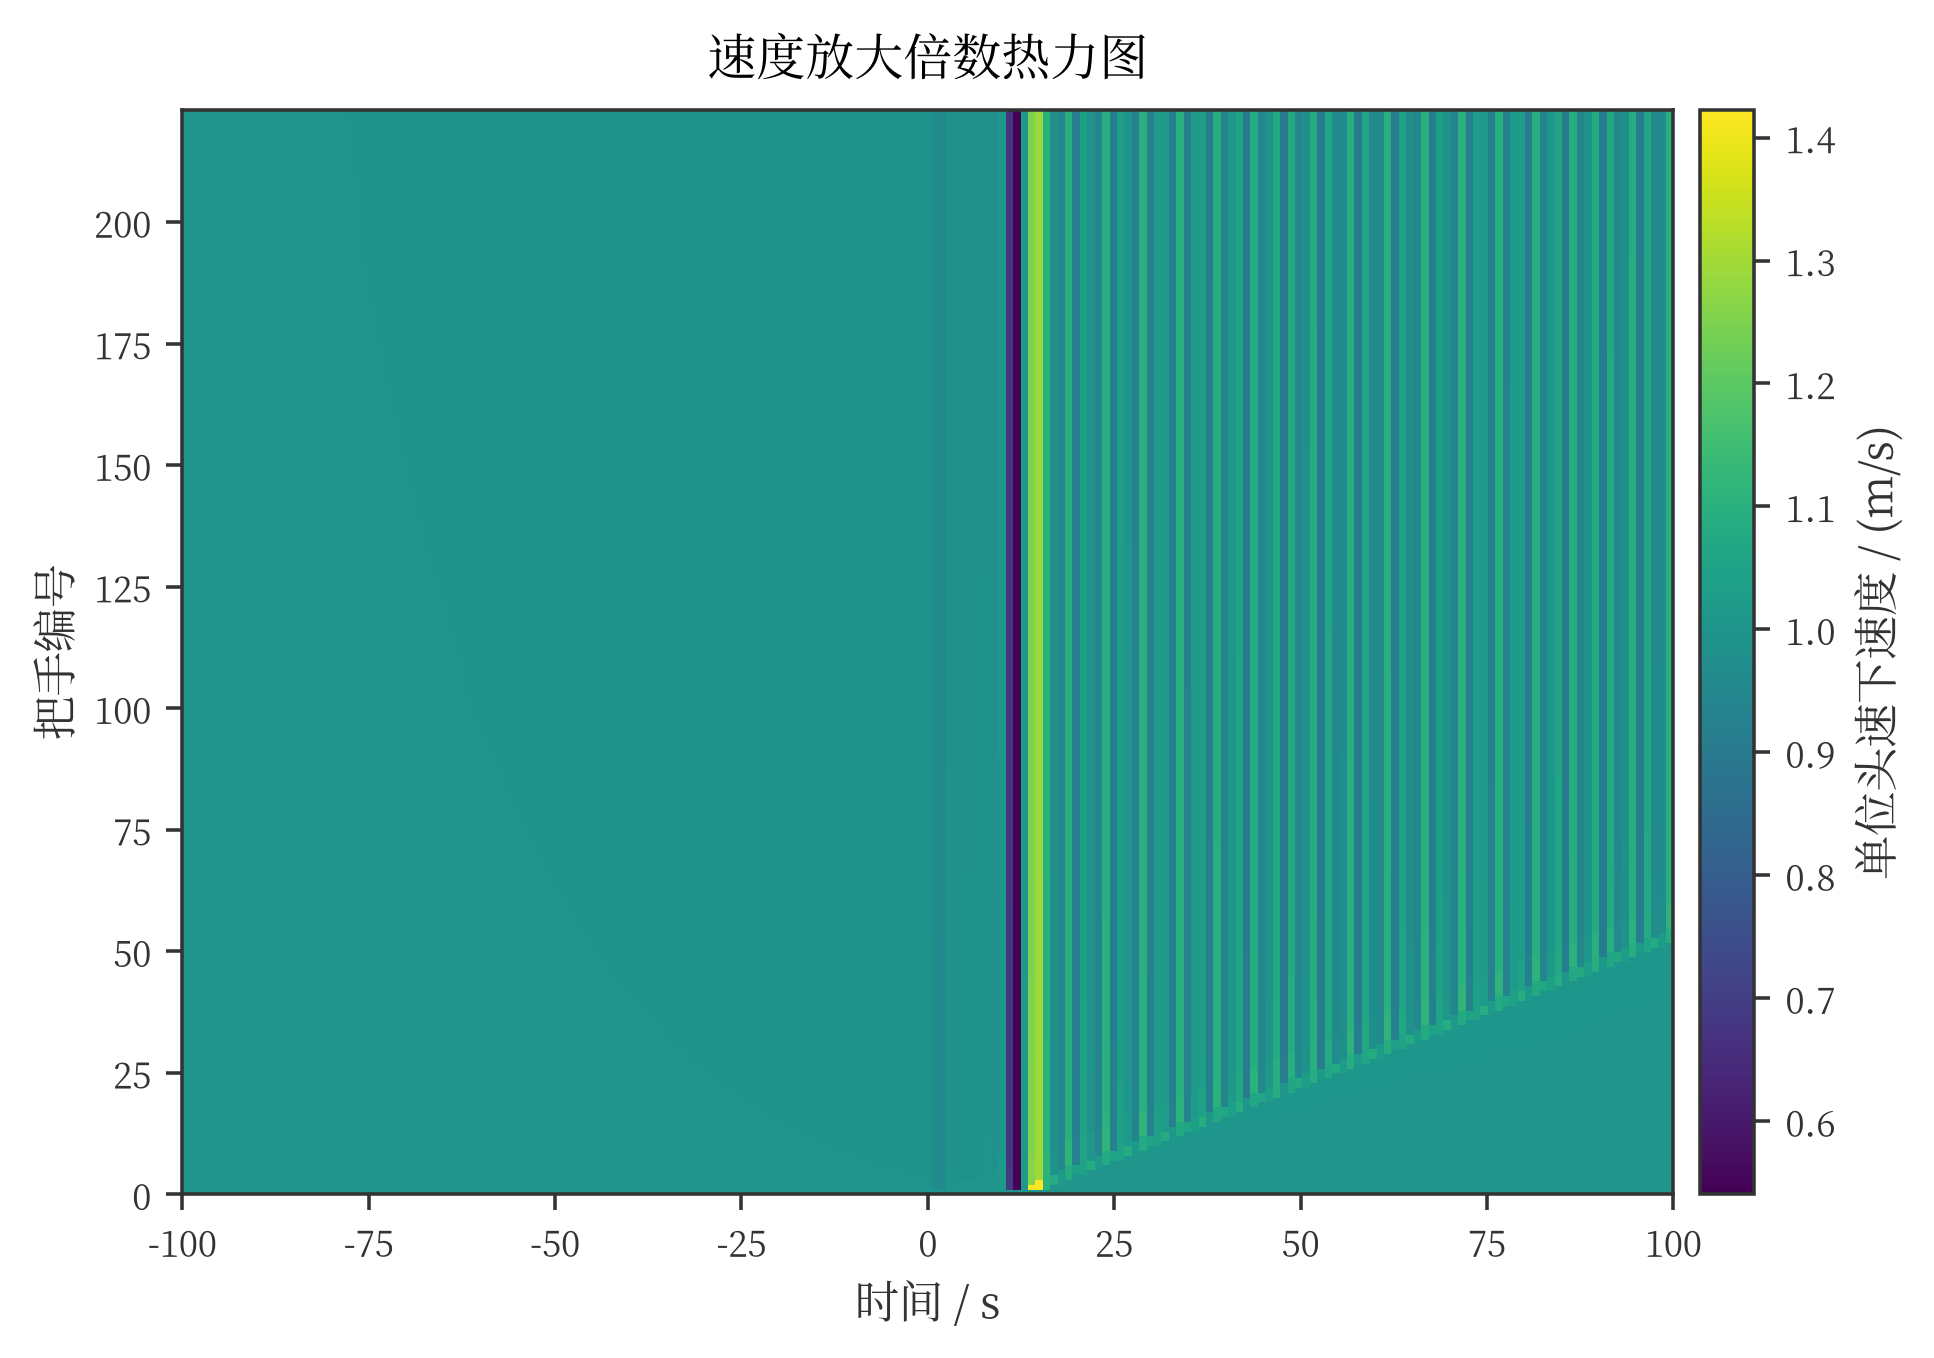
\includegraphics[width=0.9\textwidth]{figures/python/q5_speed_factor_heatmap.png}
\caption{单位头速下速度放大倍数热力图}
\label{fig:q5-speed-factor-heatmap}
\end{figure}

\subsection{求解过程}
求解时，首先读取问题四已经确定的固定交点复合路径；随后在$-100$到$100$ s的整数时刻上，按相邻把手距离约束递推全部把手位置；再根据切向投影关系计算单位头速下的速度矩阵。最后从该矩阵中提取$\lambda_{\max}$、限制时刻和限制把手，并代入$v_{\max}=2/\lambda_{\max}$得到龙头速度上界。

\begin{algorithm}[H]
\caption{问题五最大恒定头速反推流程}
\label{alg:q5-speed}
\textbf{Input:} 问题四固定调头路径，最大允许把手速度$2$ m/s。\\
\textbf{Output:} 龙头最大恒定速度$v_{\max}$。
\begin{enumerate}[label=\arabic*:, leftmargin=2.6em, itemsep=0.2em]
\item 由固定交点和两段相切圆弧构造复合路径。
\item 对每个整数时刻$t\in[-100,100]$，递推求解全部把手位置。
\item 在单位头速下递推计算各把手速度。
\item 取速度矩阵中的最大值作为$\lambda_{\max}$。
\item 根据$v_{\max}=2/\lambda_{\max}$反推龙头速度上界。
\item \textbf{return} $v_{\max}$。
\end{enumerate}
\end{algorithm}

\subsection{结果分析}
最终得到的最大恒定头速为
\[
v_{\max}=1.406\ \text{m/s},
\]
对应最大放大倍数为$1.422$。在该速度下，全队最大把手速度为
\[
2.000\ \text{m/s},
\]
满足题目要求。

单位头速速度矩阵中的最大值出现在$t=14$ s，对应限制把手为第1节龙身。也就是说，龙头速度继续增大时，该把手将最先达到2 m/s的速度上限，因此它决定了本问的最大恒定头速。

\begin{table}[H]
\centering
\caption{问题五速度上界结果表}
\label{tab:q5-result}
\begin{tabularx}{0.86\textwidth}{LCC}
\toprule
量 & 数值 & 单位\\
\midrule
最大恒定头速 & 1.406 & m/s\\
最大放大倍数 & 1.422 & --\\
限制时刻 & 14 & s\\
限制把手 & 第1节龙身 & --\\
缩放后最大把手速度 & 2.000 & m/s\\
\bottomrule
\end{tabularx}
\end{table}

\subsection{小结}
问题五是一个在固定几何路径上的速度约束反推问题。通过单位头速下的速度矩阵，可以同时得到最大速度放大倍数、限制时刻和限制把手；再由2 m/s的速度上限反推龙头恒定速度。该处理方式与问题四的固定交点路径保持同一几何口径，也使最终速度上界具有明确的约束来源。

\section{结果讨论}
表\ref{tab:summary}汇总了五个问题的核心结果。可以看出，这组题目并不是五个彼此独立的数值任务，而是同一条几何主线上的连续推进：Q1负责把“运动”变成可计算的参数递推，Q2把“是否碰撞”变成矩形交叠判定，Q3把“最小螺距”变成角点到板凳轴线距离的临界搜索，Q4把“调头路径”变成固定交点下的两圆弧几何构造，Q5则把“速度上限”变成比例缩放下的约束反推。

\begin{table}[H]
\centering
\caption{五个问题的核心结果汇总}
\label{tab:summary}
\begin{tabularx}{\textwidth}{>{\centering\arraybackslash}p{0.12\textwidth}L}
\toprule
问题 & 核心结果 \\
\midrule
Q1 & 0--300 s全把手轨迹生成完成，最大相邻把手距离误差为$8.32\times10^{-12}$ m \\
Q2 & 无碰撞终止时刻为$412.474$ s，首个碰撞板对为$[0,8]$ \\
Q3 & 最小螺距为$0.45$ m，粗扫触发螺距为$d=0.45$ m \\
Q4 & 固定交点两圆弧调头路径长度为$13.621$ m \\
Q5 & 固定交点路径下最大恒定速度为$1.406$ m/s \\
\bottomrule
\end{tabularx}
\end{table}

从结果稳定性看，Q1、Q2、Q3和Q4都具有明确的边界检验或区间逼近结构，因此数值结论较为稳定。Q5建立在问题四固定路径的速度矩阵之上，其速度上界由单位头速下的最大速度放大倍数直接给出。

从方法一致性看，全文始终使用同一套把手间距和几何递推框架，这一点避免了“Q1按中心线算、Q2按实体算”造成的逻辑断裂。尤其是Q3和Q5，都直接建立在前序问题给出的几何约束之上，因此它们的结论必须与前序问题保持同一解释口径。

\section{结论}
本文围绕“板凳龙”运动过程建立了统一的几何建模框架。首先，利用等距螺线弧长参数化与逐节递推，完成了盘入阶段全把手状态的精确恢复；随后，引入有限宽度矩形碰撞模型，求得无碰撞终止时刻；进一步以螺线与调头圆的交点为入点，在调头空间内构造两段相切圆弧；最后通过速度比例缩放，得到满足全队速度约束的最大恒定龙头速度。

本文的主要结论可以概括为四点：其一，等距螺线加弧长递推能够稳定描述板凳龙的连续运动；其二，有限宽度矩形模型比中心线模型更适合判定盘入阶段的碰撞边界；其三，Q3在角点到板凳轴线距离判据下给出的最小螺距约为$0.45$ m；其四，固定交点调头路径下的龙头最大恒定速度为$1.406$ m/s。

因此，本文给出的不是一组孤立数值，而是一套可复用的建模流程：先定路径，再定约束，最后在统一几何框架下完成搜索、判定与反推。这个流程与题目要求是一一对应的，也为后续类似板式编队运动问题提供了可迁移的思路。


\begin{thebibliography}{9}
\bibitem{cumcm2024a}
全国大学生数学建模竞赛组委会.
2024高教社杯全国大学生数学建模竞赛A题：板凳龙闹元宵及附件[Z].
2024.

\bibitem{cumcmthesis}
latexstudio.
CUMCMThesis：全国大学生数学建模竞赛\LaTeX{}论文模板[EB/OL].
\url{https://github.com/latexstudio/CUMCMThesis}.

\bibitem{ericson2005}
Ericson C.
Real-Time Collision Detection[M].
Boca Raton: CRC Press, 2005.

\bibitem{burden2015}
Burden R L, Faires J D, Burden A M.
Numerical Analysis[M].
10th ed.
Boston: Cengage Learning, 2015.
\end{thebibliography}

\begin{appendices}
\section{主要程序清单}
本文附录主要代码采用\path{ref_code/}目录下的可读Python脚本。该目录中部分以\path{.py}结尾的文件实际为Excel或压缩文件，故不作为源码插入；用于复现实验口径的主要脚本如表\ref{tab:appendix-code-files}所示。

\begin{table}[H]
\centering
\caption{主要程序文件说明}
\label{tab:appendix-code-files}
\begin{tabularx}{\textwidth}{cLL}
\toprule
对应内容 & 程序文件 & 作用说明\\
\midrule
运动递推与问题一表格 & \path{ref_code/24A_Q1.py} & 龙头角度反解、逐节把手位置递推和速度输出\\
碰撞搜索与问题二表格 & \path{ref_code/24A_Q2.py} & 板凳几何关系、碰撞距离判定和终止状态输出\\
螺距搜索 & \path{ref_code/24A_Q3.py} & 掉头边界约束下的螺距可行性判断与二分搜索\\
调头与速度约束 & \path{ref_code/24A_Q4.py} & 双圆弧调头路径、盘入盘出状态和速度约束计算\\
补充参考程序 & \path{ref_code/solution3.py} & 参考代码中的补充求解程序\\
\bottomrule
\end{tabularx}
\end{table}

\section{主要代码}
以下给出\path{ref_code/}目录中可读的主要Python代码。代码清单采用CUMCMThesis模板附录中的\texttt{listings}格式排版。

\subsection{运动递推与问题一表格程序}
\lstinputlisting[style=mcmpython,caption={运动递推与问题一表格程序},label={code:ref-q1}]{../ref_code/24A_Q1.py}

\subsection{碰撞搜索与问题二表格程序}
\lstinputlisting[style=mcmpython,caption={碰撞搜索与问题二表格程序},label={code:ref-q2}]{../ref_code/24A_Q2.py}

\subsection{螺距搜索程序}
\lstinputlisting[style=mcmpython,caption={螺距搜索程序},label={code:ref-q3}]{../ref_code/24A_Q3.py}

\subsection{调头路径与速度约束程序}
\lstinputlisting[style=mcmpython,caption={调头路径与速度约束程序},label={code:ref-q4}]{../ref_code/24A_Q4.py}

\subsection{补充参考程序}
\lstinputlisting[style=mcmpython,caption={补充参考程序},label={code:ref-solution3}]{../ref_code/solution3.py}
\end{appendices}
\end{document}
